\chapter{Marco Teórico} \label{chapter:II}
\begin{spacing}{1.5}
\section{Open Source}
		Traducito literalemte como "fuente abierta", refiri\'{e}ndose as\'{i} a una caracter\'{i}stica del software donde el c\'{o}digo fuente es de libre acceso, sin embargo, Open Source no solo significa eso. Los t\'{e}rminos de distribuci\'{o}n de un software Open Source deben cumplir con los siguientes criterios:

		\begin{enumerate}
			\item \textbf{Distribuci\'{o}n gratuita}\\
			La licencia no impedirá a ninguna parte vender o regalar el software como un componente de una distribución de software agregada que contenga programas de varias fuentes diferentes. La licencia no requerirá regalías u otros honorarios por dicha venta \cite{chap2_open_source}.
			
			\item \textbf{C\'{o}digo fuente}\\
			El programa debe incluir el código fuente y debe permitir la distribución en código fuente y en forma compilada. Cuando alguna forma de un producto no se distribuye con el código fuente, debe haber un medio que est\'{e} bien publicitado para obtener el código fuente por un costo de reproducción no superior al razonable, preferiblemente, descargarlo a través de Internet sin cargo. El código fuente debe ser la forma preferida en la que un programador modificaría el programa. No se permite el código fuente deliberadamente ofuscado. No se permiten formas intermedias como la salida de un preprocesador o traductor \cite{chap2_open_source}.

			\item \textbf{Trabajos derivados}\\
			La licencia debe permitir modificaciones y trabajos derivados, y debe permitir que se distribuyan en los mismos términos que la licencia del software original \cite{chap2_open_source}.
			
			\item \textbf{Integridad del autor del c\'{o}digo fuente}\\
			La licencia puede restringir la distribución del código fuente en forma modificada solo si la licencia permite la distribución de "archivos de parche" con el código fuente con el fin de modificar el programa en el momento de la compilación. La licencia debe permitir explícitamente la distribución de software creado a partir del código fuente modificado. La licencia puede requerir que las obras derivadas lleven un nombre o número de versión diferente al del software original \cite{chap2_open_source}.
			
			\item \textbf{No discriminaci\'{o}n contra persona y grupos}\\
			La licencia no debe discriminar a ninguna persona o grupo de personas \cite{chap2_open_source}.
			
			\item \textbf{No discrininaci\'{o}n en los lugares de actividad}\\
			La licencia no debe restringir a nadie el uso del programa en un campo específico de actividad. Por ejemplo, no puede restringir el uso del programa en una empresa o para la investigación genética \cite{chap2_open_source}.
			
			\item \textbf{Licencia de distribuci\'{o}n}\\
			Los derechos adjuntos al programa deben aplicarse a todos aquellos a quienes se redistribuye el programa sin la necesidad de que esas partes ejecuten una licencia adicional \cite{chap2_open_source}.
			
			\item \textbf{La licencia no debe ser espec\'{i}fica para un producto}\\
			Los derechos adjuntos al programa no deben depender de que el programa sea parte de una distribución de software en particular. Si el programa se extrae de esa distribución y se usa o distribuye dentro de los términos de la licencia del programa, todas las partes a quienes se redistribuye el programa deben tener los mismos derechos que los que se otorgan junto con la distribución original del software \cite{chap2_open_source}.
			
			\item \textbf{La licencia no debe restringir a otro software}\\
			La licencia no debe imponer restricciones a otro software que se distribuya junto con el software con licencia. Por ejemplo, la licencia no debe insistir en que todos los demás programas distribuidos en el mismo medio deben ser software de código abierto \cite{chap2_open_source}.
			
			\item \textbf{La licencia debe ser de tecnología neutral}\\
			Ninguna disposición de la licencia puede basarse en una tecnología individual o estilo de interfaz \cite{chap2_open_source}.
			
		\end{enumerate}
	
\section{Legalidad del software}
	\subsection{Licencia}
	Una licencia es la autorización que se concede para explotar con fines industriales o comerciales una patente, marca o derecho. Diccionario de la lengua española (23.ª ed.)
	
	\subsection{Derecho de autor o Copyright}
	Derecho que la ley reconoce al autor de una obra intelectual o artística para autorizar su reproducción y participar en los beneficios que esta genere. Diccionario de la lengua española (23.ª ed.)
	
	\subsection{Patente}
	Documento expedido por una autoridad en que se acredita una condición o un mérito o se da la autorización para hacer algo. Diccionario de la lengua española (23.ª ed.)
	
	\subsection{Licencia de Software}
	Una licencia de software es un contrato entre el licenciante (autor/titular de los derechos de explotación/distribución) y el licenciatario (usuario consumidor, profesional o empresa) del programa informático, para utilizarlo cumpliendo una serie de términos y condiciones establecidas dentro de sus cláusulas, es decir, es un conjunto de permisos que un licenciante otorga a un usuario en los que tiene la posibilidad de distribuir, usar o modificar el producto bajo una licencia determinada. Además se suelen definir los plazos de duración, el territorio donde se aplica la licencia (ya que la licencia se soporta en las leyes particulares de cada país o región), entre otros.
	
	\subsection{Licencia Open Source}
	Las licencias de código abierto son licencias que cumplen con la definición de código abierto; en resumen, permiten que el software se utilice, modifique y comparta libremente. Para ser aprobada por Open Source Initiative (también conocida como OSI), una licencia debe pasar por el proceso de revisión de licencias de Open Source Initiative.\cite{chap2_open_source_2}\\
	
	Existen 100 licencias registradas en la Open Source Initiative(OSI), de las cual el presente proyecto describi\'{a} 2 de ellas por ser las m\'{a}s importante del proyecto Saiku Analytics.

	\subsubsection{Licencia Apache}
	La licencia de Apache solo requiere un reconocimiento en la ``documentación del usuario final" o ``en el software mismo", no en ``todos los materiales publicitarios". La licencia de Apache no especifica la prominencia que debe darse a ese reconocimiento. La licencia de Apache es consistente con los Principios de código abierto porque no interfiere con la libertad de modificar o crear trabajos derivados de software de código abierto.\cite{chap2_apache_license}\\
	Se deben añadir dos archivos en el directorio principal de los paquetes de software redistribuidos.
	\begin{enumerate}
		\item LICENSE: Una copia de la licencia
		\item NOTICE: Un documento de texto que incluye los “avisos” obligatorios del software presente en la distribución y una copia legible de estas notificaciones deben ser distribuidas como parte de los trabajos derivados, dentro de la forma de código fuente o documentación, o dentro de una pantalla generada por las obras derivadas ( donde aparecen normalmente este tipo de notificaciones a terceros).
	\end{enumerate}			

	\subsubsection{Licencia MIT}
	Licencia creada por los abogados del Instituto de Tecnología de Massachusetts (MIT) a partir de la licencia BSD. Limpiaron algo del lenguaje vago de la licencia BSD y facilitaron la lectura y la comprensión de su versión. En los Apéndices se muestra una copia de la versión actual de la licencia MIT.\\
	La concesión de la licencia del MIT se extiende no solo al software en sí, sino a sus archivos de documentación asociados. No está claro si el MIT se ofrece aquí para proporcionar toda la documentación en su poder sobre el software o solo ciertos archivos que están asociados de alguna manera con el software.\\
	La frase sin cargo significa que el licenciante (MIT en este caso) no cobrará regalías o derechos de licencia. Pero la palabra vender entre la lista de derechos otorgados significa que los licenciatarios posteriores no están restringidos de ninguna manera para cobrar regalías o tarifas de licencia a sus clientes por versiones modificadas del software.\\
	La licencia del MIT también sirve como plantilla de licencia. Es una licencia tan corta que solo es necesario cambiar el aviso de derechos de autor para completar la plantilla. Desafortunadamente, la frase este software y los archivos de documentación asociados no identifican claramente a qué software se aplica la licencia. La única forma de correlacionar un software en particular con una copia particular de la licencia del MIT es encontrar físicamente el texto de la licencia en el código fuente del software.\cite{chap2_MIT_license}\\
	
%------------------------------------------------------------------------------------------------------------------
%------------------------------------- Saiku Analytics ------------------------------------------------------------
%------------------------------------------------------------------------------------------------------------------	
\section{Saiku Analytics}
	Saiku fue fundada en 2008 por Tom Barber y Paul Stoellberger. Originalmente llamada \textit{Pentaho Analysis Tool}, comenzó como un contenedor básico basado en GWT alrededor de la biblioteca OLAP4J. A lo largo de los años ha evolucionado, y después de una reescritura completa en 2010, renació como Saiku.
	
	Saiku ofrece una solución de análisis basada en web fácil de usar que permite a los usuarios analizar rápida y fácilmente los datos corporativos y crear y compartir informes. La solución se conecta a una variedad de servidores OLAP, incluidos Mondrian, Microsoft Analysis Services, SAP BW y Oracle Hyperion y se puede implementar de manera rápida y rentable para permitir a los usuarios explorar datos en tiempo real.
	
	Saiku es una popular herramienta de análisis gráfico de código abierto para Mondrian que se puede ejecutar de forma independiente o como un complemento de Pentaho \cite{chap2_mondrian_action}.
	
	\subsection{Pentaho}
	Son una plataforma integral que se utilizan para acceder, integrar, manipular, visualizar y analizar datos. Ya sea que los datos se almacenen en un archivo plano, una base de datos relacional, un clúster Hadoop, una base de datos NoSQL, una base de datos analítica, transmisiones de redes sociales, tiendas operativas o en la nube, los productos Pentaho pueden ayudarlo a descubrir, analizar y visualizar datos para encontrar las respuestas que necesita, incluso si no tiene experiencia en codificación. Los usuarios avanzados con experiencia en programación pueden utilizar la extensa API para personalizar informes, consultas y transformaciones para ampliar la funcionalidad.\\
	Los productos de Pentaho incluyen tanto componentes basados en web como herramientas de diseño. Los componentes y herramientas que utiliza dependen de su flujo de trabajo y de lo que admita su entorno \cite{chap2_pentaho}.
	\subsubsection{Web-based Components}
	Son componentes basados en la web de Pentaho creados para compartir soluciones de inteligencia empresarial mediante el a\'{a}lisis de datos la creaci\'{o}n de informes y de paneles integrados.
		\begin{enumerate}[label=\alph*)]
			\item \textbf{Consola de usuario}\\
			La Consola de usuario de Pentaho (PUC) es un entorno de diseño para acceder a Analyzer, Reportes interactivos y Dashboard Designer. La consola de usuario de Pentaho también ofrece funciones de administración del sistema para configurar su servidor Pentaho \cite{chap2_pentaho}.
			
			\item \textbf{Analizador}\\
			Analyzer lo ayuda a visualizar datos para tomar decisiones comerciales informadas. Puede crear visualizaciones geográficas, gráficas de dispersión, cuadrículas térmicas y de múltiples gráficas. También puede filtrar datos, agregar parámetros de consulta, configurar enlaces detallados, aplicar formato condicional y generar hipervínculos \cite{chap2_pentaho}.
			
			\item \textbf{Informes interactivos}\\
			Interactive Reports es una interfaz de diseño que se utiliza para crear informes operativos simples y bajo demanda sin depender de TI o desarrolladores de informes. Puede agregar elementos rápidamente a su informe y aplicarles el formato que desee \cite{chap2_pentaho}.
			
			\item \textbf{Diseñador de paneles}\\
			Dashboard Designer se utiliza para elegir plantillas de diseño, temas y contenido para crear paneles visualmente atractivos que ayuden a los tomadores de decisiones a obtener conocimientos críticos de un vistazo. Puede combinar una amplia variedad de contenido, incluidos informes interactivos, visualizaciones del analizador y contenido colaborativo \cite{chap2_pentaho}.
			
			\item \textbf{CTools}\\
			CTools es un marco impulsado por la comunidad para crear paneles mediante el uso de tecnologías web como JavaScript, CSS y HTML. Puede crear fácilmente cuadros de mando dinámicos para que los usuarios exploren y comprendan grandes cantidades de datos mediante una variedad de gráficos, tablas y otros componentes \cite{chap2_pentaho}.
			
			\item \textbf{Asistente de fuente de datos}\\
			El Asistente de fuente de datos lo ayuda a definir una fuente de datos que contiene su información y lo guía a través de la creación de sus primeros modelos relacionales o multidimensionales para usar en la creación de informes y análisis \cite{chap2_pentaho}.
			
			\item \textbf{Editor de modelos de fuente de datos}\\
			El Editor de modelos de origen de datos le ayuda a ajustar y perfeccionar los modelos de datos relacionales y multidimensionales. Puede arrastrar campos a sus ubicaciones apropiadas, mezclar y combinar campos de diferentes tablas, agregar campos a más de una categoría o eliminar un campo \cite{chap2_pentaho}.
		\end{enumerate}
	\subsubsection{Design Tools}
	Las herramientas de diseño de Pentaho son para desarrollar y perfeccionar cómo se informan, modelan, transforman y almacenan los valores de sus datos.
		\begin{enumerate}
			\item \textbf{Integración de datos}\\
			Pentaho Data Integration (PDI) brinda acceso a un motor de extracción, transformación y carga (ETL) que captura los datos correctos, los limpia y los almacena utilizando un formato uniforme que es accesible y relevante para los usuarios finales y las tecnologías de IoT \cite{chap2_pentaho}.
			
			\item \textbf{Diseñador de informes}\\
			Report Designer se utiliza para generar informes detallados con píxeles perfectos utilizando prácticamente cualquier fuente de datos. Permite a los profesionales de inteligencia empresarial crear informes de calidad de impresi\'{o}n altamente detallados y basados en datos preparados adecuadamente \cite{chap2_pentaho}.
		
			\item \textbf{Diseñador de agregaciones}\\
			Aggregation Designer proporciona una interfaz simple que le permite crear tablas agregadas a partir de niveles dentro de las dimensiones que especifique. Utilice esta herramienta para mejorar el rendimiento de sus cubos OLAP de Pentaho Analysis (Mondrian) \cite{chap2_pentaho}.
			
			\item \textbf{Editor de metadatos}\\
			Metadata Editor simplifica la creación de informes. Utilice el editor de metadatos para crear modelos y dominios de metadatos de Pentaho. Un modelo de metadatos de Pentaho mapea la estructura física de su base de datos en un modelo de negocio lógico \cite{chap2_pentaho}.
			
			\item \textbf{Schema Workbench}\\
			Schema Workbench le permite editar y crear modelos multidimensionales (Mondrian). Puede crear modelos de Mondrian gráficamente o definirlos codificando manualmente archivos XML \cite{chap2_pentaho}.
		\end{enumerate}
%------------------------------------------------------------------------------------------------------------------
%-------------------------------------  SCRUM  --------------------------------------------------------------------
%------------------------------------------------------------------------------------------------------------------
\section{SCRUM}
	\subsection{Definici\'{o}n de Scrum}
		Scrum es un marco de trabajo liviano que ayuda a las personas, equipos y organizaciones a generar valor
		a través de soluciones adaptativas para problemas complejos \cite{chap2_scrum}.\\
		El marco de trabajo Scrum es incompleto de manera intencional, solo define las
		partes necesarias para implementar la teoría de Scrum. Scrum se basa en la inteligencia colectiva de las
		personas que lo utilizan. En lugar de proporcionar a las personas instrucciones detalladas, las reglas de
		Scrum guían sus relaciones e interacciones.\\
		En este marco de trabajo pueden emplearse varios procesos, técnicas y métodos. Scrum envuelve las
		prácticas existentes o las hace innecesarias. Scrum hace visible la eficacia relativa de las técnicas
		actuales de gestión, entorno y trabajo, de modo que se puedan realizar mejoras.
	\subsection{Teor\'{i}a de Scrum}
		Scrum se basa en el empirismo y el pensamiento Lean. El empirismo afirma que el conocimiento
		proviene de la experiencia y de la toma de decisiones con base en lo observado. El pensamiento Lean
		reduce el desperdicio y se enfoca en lo esencial.\\
		Scrum emplea un enfoque iterativo e Incremental para optimizar la previsibilidad y controlar el riesgo.
		Scrum involucra a grupos de personas que colectivamente tienen todas las habilidades y experiencia
		para hacer el trabajo y compartir o adquirir dichas habilidades según sea necesario.
		Scrum combina cuatro eventos formales para inspección y adaptación dentro de un evento contenedor,
		el Sprint. Estos eventos funcionan porque implementan los pilares empíricos de Scrum de transparencia,
		inspección y adaptación \cite{chap2_scrum}.
		\subsubsection{Transparencia}
			El proceso y el trabajo emergentes deben ser visibles tanto para quienes realizan el trabajo como para
			quienes lo reciben. Con Scrum, las decisiones importantes se basan en el estado percibido de sus tres artefactos formales. Los artefactos que tienen poca transparencia pueden llevar a decisiones que
			disminuyan el valor y aumenten el riesgo.\\
			La transparencia permite la inspección. La inspección sin transparencia es engañosa y derrochadora \cite{chap2_scrum}.
		\subsubsection{Inspecci\'{o}n}
			Los artefactos de Scrum y el progreso hacia los objetivos acordados deben inspeccionarse con
			frecuencia y con diligencia para detectar variaciones o problemas potencialmente indeseables. Para
			ayudar con la inspección, Scrum proporciona cadencia en forma de sus cinco eventos.\\
			La inspección permite la adaptación. La inspección sin adaptación se considera inútil. Los eventos Scrum
			están diseñados para provocar cambios \cite{chap2_scrum}.
		\subsubsection{Adaptaci\'{o}n}
			Si algún aspecto de un proceso se desvía fuera de los límites aceptables o si el producto resultante es
			inaceptable, el proceso que se aplica o los materiales que se producen deben ajustarse. El ajuste debe
			realizarse lo antes posible para minimizar una mayor desviación.\\
			La adaptación se vuelve más difícil cuando las personas involucradas no están empoderadas ni se
			autogestionan. Se espera que un Scrum Team se adapte en el momento en que aprenda algo nuevo a
			través de la inspección \cite{chap2_scrum}.
	\subsection{Valores de Scrum}
			El uso exitoso de Scrum depende de que las personas se vuelvan más competentes en vivir cinco valores: \textbf{Compromiso, Foco, Franqueza, Respeto y Coraje}.
			El Scrum Team se compromete a lograr sus objetivos y a apoyarse mutuamente. Su foco principal está
			en el trabajo del Sprint para lograr el mejor progreso posible hacia estos objetivos. El Scrum Team y sus interesados son francos sobre el trabajo y los desafíos. Los miembros del Scrum Team se respetan entre sí para ser personas capaces e independientes, y son respetados como tales por las personas con las que	trabajan. Los miembros del Scrum Team tienen el coraje de hacer lo correcto, para trabajar en
			problemas difíciles \cite{chap2_scrum}.\\
			Estos valores dan dirección al Scrum Team con respecto a su trabajo, acciones y comportamiento. Las
			decisiones que se tomen, los pasos que se den y la forma en que se use Scrum deben reforzar estos
			valores, no disminuirlos ni socavarlos. Los miembros del Scrum Team aprenden y exploran los valores
			mientras trabajan con los eventos y artefactos Scrum. Cuando el Scrum Team y las personas con las que trabajan incorporan estos valores, los pilares empíricos de Scrum de transparencia, inspección y 		adaptación cobran vida y generan confianza.
	\subsection{\textit{Scrum Team}}
		La unidad fundamental de Scrum es un pequeño equipo de personas, un \textit{Scrum Team}. El \textit{Scrum Team} consta de un \textit{Scrum Master}, un \textit{Product Owner} y \textit{Developers}. Dentro de un \textit{Scrum Team}, no hay subequipos ni jerarquías. Es una unidad cohesionada de profesionales enfocados en un objetivo a la vez, el Objetivo del Producto.
		Los \textit{Scrum Teams} son multifuncionales, lo que significa que los miembros tienen todas las habilidades
		necesarias para crear valor en cada \textit{Sprint}. También se autogestionan, lo que significa que deciden
		internamente quién hace qué, cuándo, cómo y porqu\'{e} \cite{chap2_scrum}.\\
		El \textit{Scrum Team} es lo suficientemente pequeño como para seguir siendo ágil y lo suficientemente grande
		como para completar un trabajo significativo dentro de un Sprint, generalmente 10 personas o menos.
		En general, hemos descubierto que los equipos más pequeños se comunican mejor y son más
		productivos. Si los \textit{Scrum Teams} se vuelven demasiado grandes, deberían considerar reorganizarse en
		múltiples \textit{Scrum Teams} cohesivos, cada uno enfocado en el mismo producto. Por lo tanto, deben
		compartir el mismo Objetivo del Producto, el \textit{Product Backlog} y el \textit{Product Owner}.
		El \textit{Scrum Team} es responsable de todas las actividades relacionadas con el producto, desde la
		colaboración de los interesados, la verificación, el mantenimiento, la operación, la experimentación, la
		investigación y el desarrollo, y cualquier otra cosa que pueda ser necesaria. Están estructurados y
		empoderados por la organización para gestionar su propio trabajo. Trabajar en \textit{Sprints} a un ritmo
		sostenible mejora el enfoque y la consistencia del \textit{Scrum Team} \cite{chap2_scrum}.
		Todo el Scrum Team es responsable de crear un Increment valioso y útil en cada Sprint. Scrum define
		tres responsabilidades específicas dentro del Scrum Team: los \textit{Developers}, el \textit{Product Owner} y el \textit{Scrum Master}.
		\subsubsection{\textit{Developers}}
			Son Las personas del \textit{Scrum Team} que se comprometen a crear cualquier aspecto de un \textit{Increment} utilizable en cada \textit{Sprint} son \textit{Developers}.
			Las habilidades específicas que necesitan los \textit{Developers} suelen ser amplias y variarán según el ámbito
			de trabajo. Sin embargo, los \textit{Developers} siempre son responsables de:
			\begin{itemize}
				\item Crear un plan para el \textit{Sprint}, el \textit{Sprint Backlog};
				\item Inculcar calidad al adherirse a una Definición de Terminado;
				\item Adaptar su plan cada día hacia el Objetivo del \textit{Sprint}; y,
				\item Responsabilizarse mutuamente como profesionales.
			\end{itemize}
		\subsubsection{\textit{Product Owner}}
			El \textit{Product Owner} es responsable de maximizar el valor del producto resultante del trabajo del \textit{Scrum Team}. La forma en que esto se hace puede variar ampliamente entre organizaciones, \textit{Scrum Teams} e individuos.\\
			El \textit{Product Owner} también es responsable de la gestión efectiva del \textit{Product Backlog}, lo que incluye:
			\begin{itemize}
				\item Desarrollar y comunicar explícitamente el Objetivo del Producto;
				\item Crear y comunicar claramente los elementos del \textit{Product Backlog};
				\item Ordenar los elementos del \textit{Product Backlog}; y,
				\item Asegurarse de que el \textit{Product Backlog} sea transparente, visible y se entienda.
			\end{itemize}
			El \textit{Product Owner} puede realizar el trabajo anterior o puede delegar la responsabilidad en otros. Independientemente de ello, el \textit{Product Owner} sigue siendo el responsable de que el trabajo se realice.\\
			Para que los \textit{Product Owners} tengan éxito, toda la organización debe respetar sus decisiones. Estas decisiones son visibles en el contenido y el orden del \textit{Product Backlog}, y a través del \textit{Increment} inspeccionable en la \textit{Sprint Review}.\\
			El \textit{Product Owner} es una persona, no un comité. El \textit{Product Owner} puede representar las necesidades de muchos interesados en el \textit{Product Backlog}. Aquellos que quieran cambiar el \textit{Product Backlog} pueden hacerlo intentando convencer al \textit{Product Owner}.
		\subsubsection{\textit{Scrum Master}}
			El Scrum Master es responsable de establecer Scrum como se define en la Guía de Scrum. Lo hace ayudando a todos a comprender la teoría y la práctica de Scrum, tanto dentro del \textit{Scrum Team} como de la organización.\\
			El \textit{Scrum Master} es responsable de lograr la efectividad del \textit{Scrum Team}. Lo hace apoyando al \textit{Scrum Team} en la mejora de sus prácticas, dentro del marco de trabajo de Scrum.\\
			Los \textit{Scrum Masters} son verdaderos líderes que sirven al \textit{Scrum Team} y a la organización en general \cite{chap2_scrum}.\\
			El \textit{Scrum Master} sirve al \textit{Scrum Team} de varias maneras, que incluyen:
			\begin{itemize}
				\item Guiar a los miembros del equipo en ser autogestionados y multifuncionales;
				\item Ayudar al \textit{Scrum Team} a enfocarse en crear \textit{Increments} de alto valor que cumplan con la``Definición de Terminado";
				\item Procurar la eliminación de impedimentos para el progreso del \textit{Scrum Team}; y,
				\item Asegurarse de que todos los eventos de Scrum se lleven a cabo y sean positivos, productivos y se mantengan dentro de los límites de tiempo recomendados en la gu\'{i}a de Scrum.
			\end{itemize}
			El \textit{Scrum Master} sirve al \textit{Product Owner} de varias maneras, que incluyen:
			\begin{itemize}
				\item Ayudar a encontrar técnicas para una definición efectiva de Objetivos del Producto y la gestión	del \textit{Product Backlog};
				\item Ayudar al \textit{Scrum Team} a comprender la necesidad de tener elementos del \textit{Product Backlog} claros y concisos;
				\item Ayudar a establecer una planificación empírica de productos para un entorno complejo; y,
				\item Facilitar la colaboración de los interesados según se solicite o necesite.
			\end{itemize}
			El Scrum Master sirve a la organización de varias maneras, que incluyen:
			\begin{itemize}
			\item Liderar, capacitar y guiar a la organización en su adopción de Scrum;
			\item Planificar y asesorar implementaciones de Scrum dentro de la organización;
			\item Ayudar a los empleados y los interesados a comprender y aplicar un enfoque empírico para el trabajo complejo; y,
			\item Eliminar las barreras entre los interesados y los \textit{Scrum Teams}.
			\end{itemize}
	\subsection{Eventos de Scrum}
		El \textit{Sprint} es un contenedor para todos los demás eventos. Cada evento en Scrum es una oportunidad formal para inspeccionar y adaptar los artefactos Scrum. Estos eventos están diseñados específicamente para habilitar la transparencia requerida. No operar cualquier evento según lo prescrito resulta en la pérdida de oportunidades para inspeccionar y adaptarse. Los eventos se utilizan en Scrum para crear regularidad y minimizar la necesidad de reuniones no definidas en Scrum.\\
		Lo óptimo es que todos los eventos se celebren al mismo tiempo y en el mismo lugar para reducir la complejidad \cite{chap2_scrum}, los eventos se pueden apreciar detalladamente en la Figura \ref{figure:chaperII_1}.
		\begin{figure}[H]
			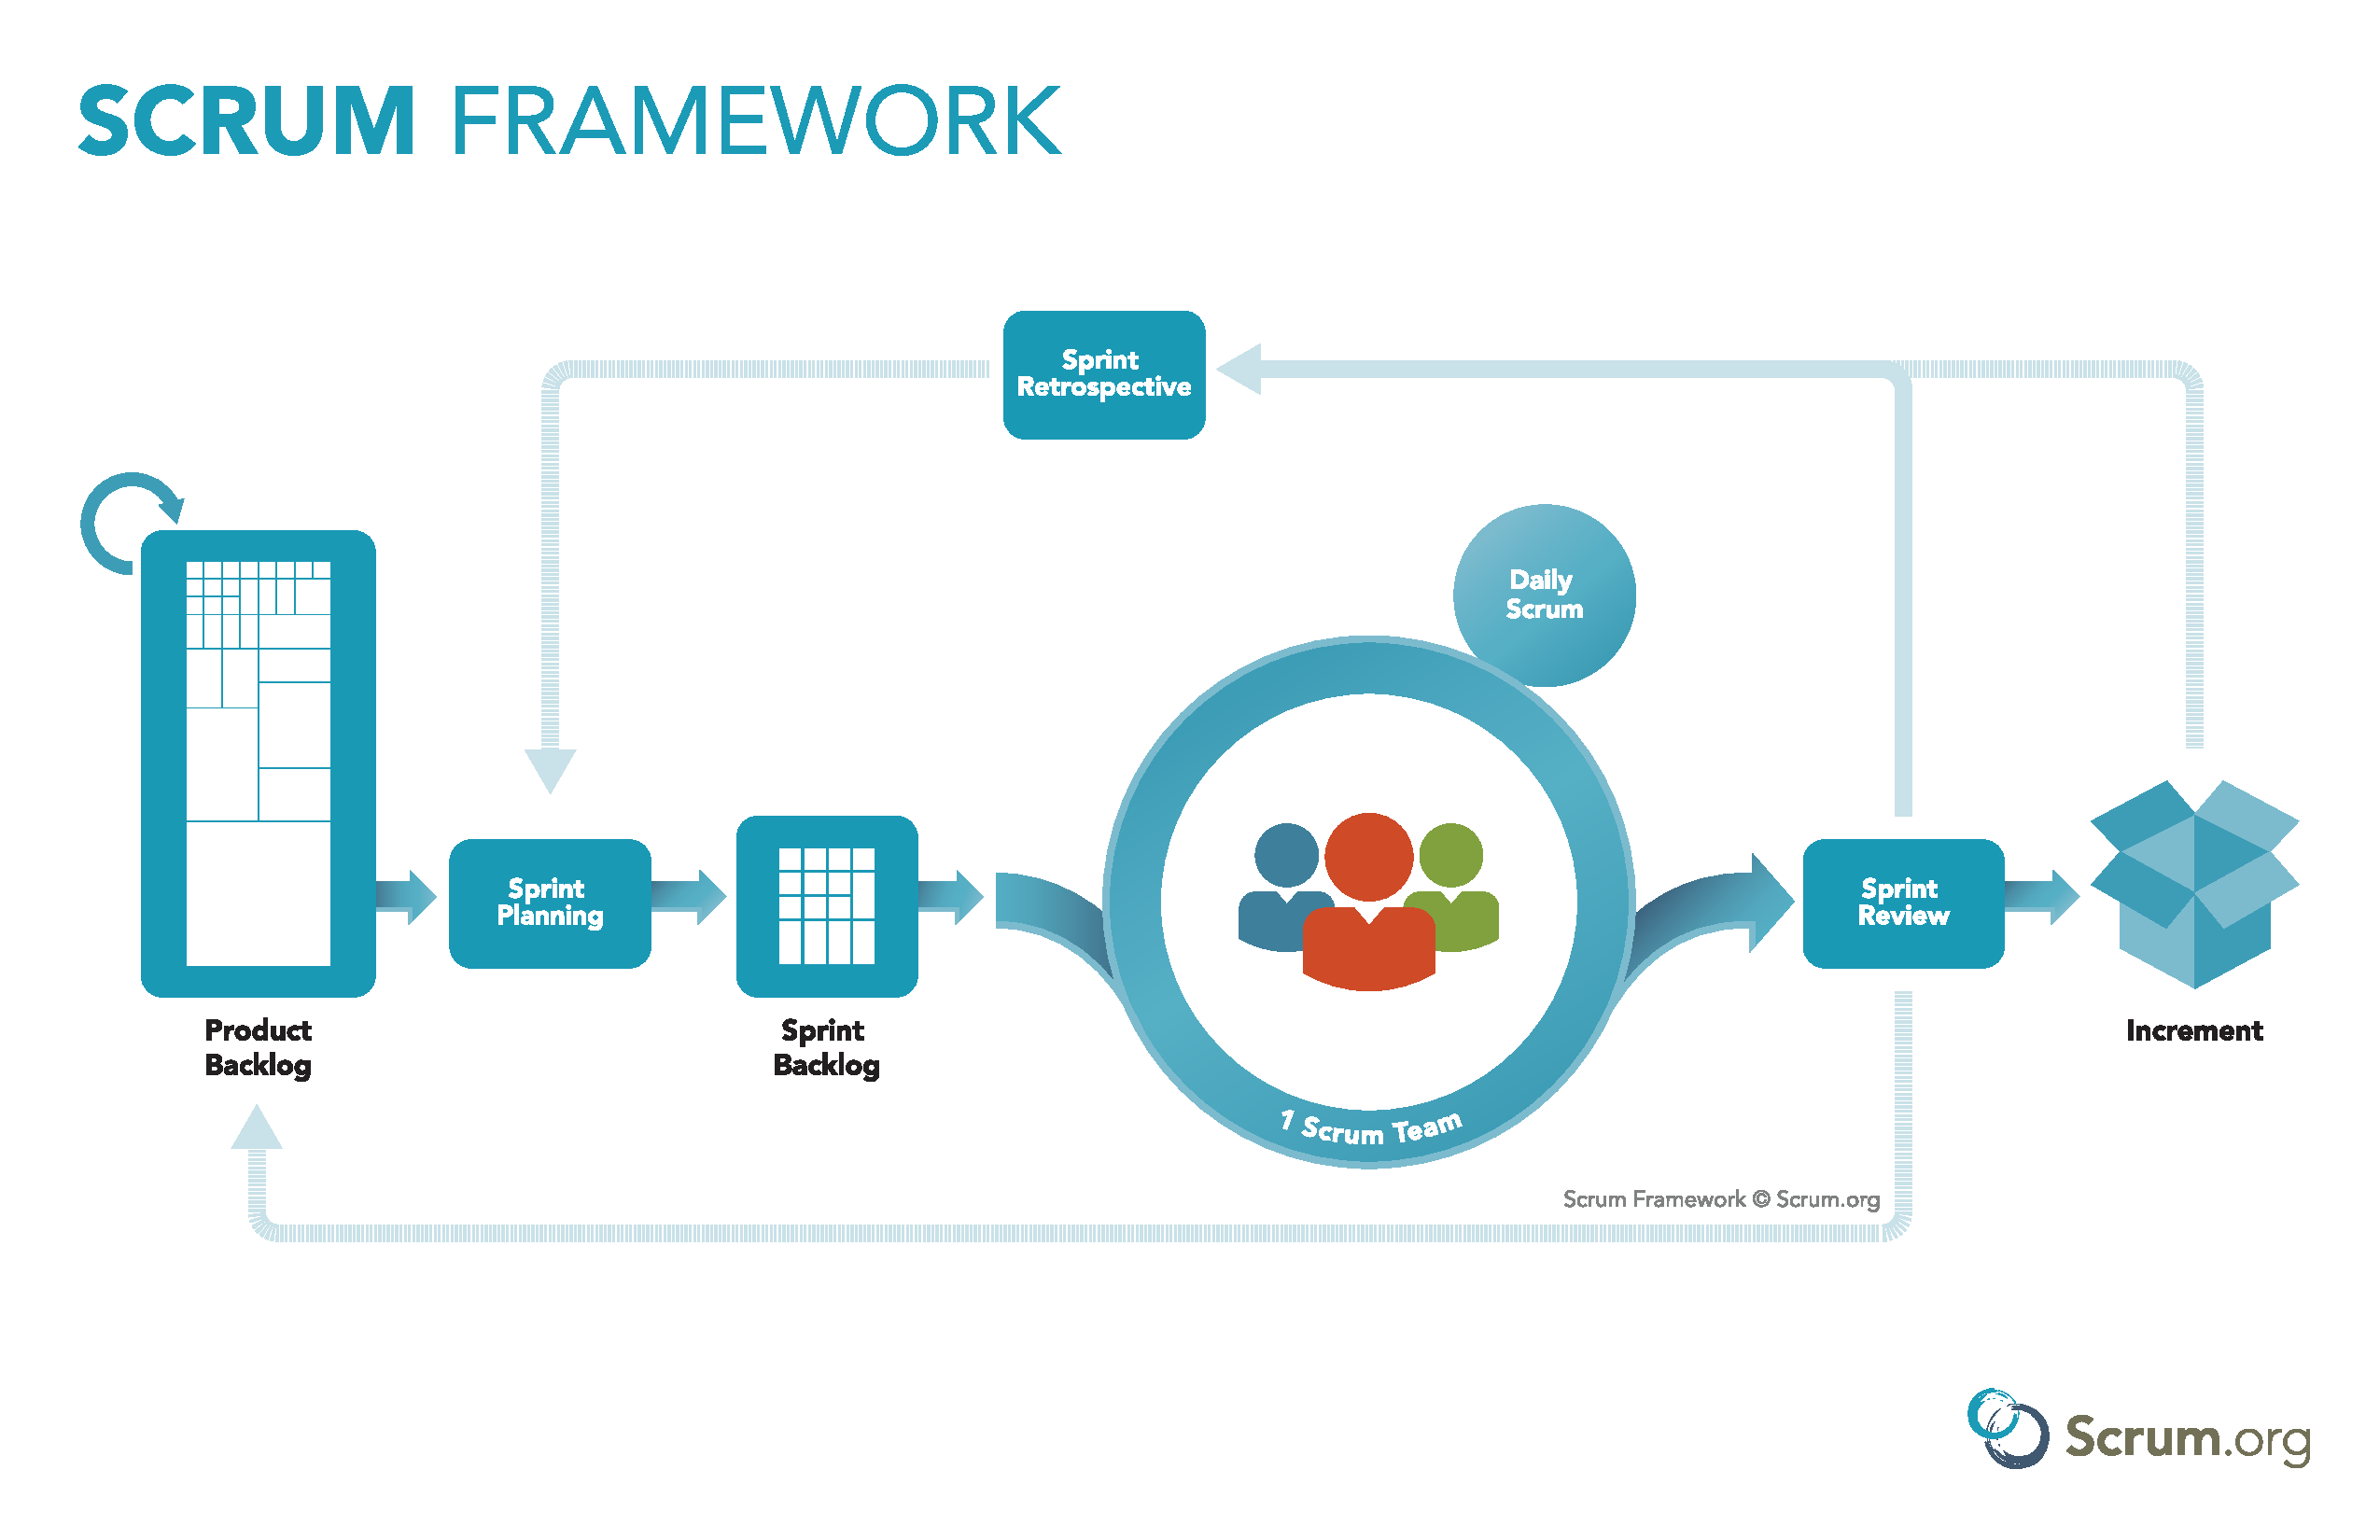
\includegraphics[page=1,width=1.0 \textwidth]{scrum.pdf}
			\caption {\centering \small{Scrum Framework}} \label{figure:chaperII_1}
			\centering \small {Nota: Extraido de ``Scrum Framework Poster", 2020, \url{www.scrum.org}}
		\end{figure}
		\subsubsection{El \textit{Sprint}}
			Los Sprints son el corazón de Scrum, donde las ideas se convierten en valor.\\
			Son eventos de duración fija de un mes o menos para crear consistencia. Un nuevo Sprint comienza inmediatamente después de la conclusión del Sprint anterior.\\
			Todo el trabajo necesario para lograr el Objetivo del Producto, incluido la \textit{Sprint Planning}, \textit{Daily Scrums}, \textit{Sprint Review} y \textit{Sprint Retrospective}, ocurre dentro de los \textit{Sprints} \cite{chap2_scrum}.\\
			Durante el Sprint:
			\begin{itemize}
				\item No se realizan cambios que pongan en peligro el Objetivo del \textit{Sprint};
				\item La calidad no disminuye;
				\item El \textit{Product Backlog} se refina según sea necesario; y,
				\item El alcance se puede aclarar y renegociar con el \textit{Product Owner} a medida que se aprende más.
			\end{itemize}
			Los \textit{Sprints} permiten la previsibilidad al garantizar la inspección y adaptación del progreso hacia un Objetivo del Producto al menos cada mes calendario. Cuando el horizonte de un \textit{Sprint} es demasiado largo, el Objetivo del \textit{Sprint} puede volverse inválido, la complejidad puede crecer y el riesgo puede aumentar. Se pueden emplear \textit{Sprints} más cortos para generar más ciclos de aprendizaje y limitar el riesgo de costo y esfuerzo a un período de tiempo menor. Cada \textit{Sprint} puede considerarse un proyecto corto.\\
			Existen varias prácticas para pronosticar el progreso, como el trabajo pendiente (\textit{burn‐downs}), trabajo completado (\textit{burn‐ups}) o flujos acumulativos (\textit{cumulative flows}). Si bien han demostrado su utilidad, no reemplazan la importancia del empirismo. En entornos complejos, se desconoce lo que sucederá. Solo lo que ya ha sucedido se puede utilizar para la toma de decisiones con miras al futuro.\\
			Un \textit{Sprint} podría cancelarse si el Objetivo del \textit{Sprint} se vuelve obsoleto. Solo el \textit{Product Owner} tiene la autoridad para cancelar el \textit{Sprint}.
		\subsubsection{\textit{Sprint Planning}}
			La \textit{Sprint Planning} inicia el \textit{Sprint} al establecer el trabajo que se realizará para el \textit{Sprint}. El \textit{Scrum Team} crea este plan resultante mediante trabajo colaborativo.\\
			El \textit{Product Owner} se asegura de que los asistentes estén preparados para discutir los elementos más importantes del \textit{Product Backlog} y cómo se relacionan con el Objetivo del Producto. El \textit{Scrum Team} también puede invitar a otras personas a asistir a la \textit{Sprint Planning} para brindar asesoramiento \cite{chap2_scrum}.\\
			El \textit{Sprint Planning} aborda los siguientes temas:
			\begin{itemize}
				\item Tema uno: ¿Por qué es valioso este \textit{Sprint}?\\
				El \textit{Product Owner} propone cómo el producto podría \textit{Incrementar} su valor y utilidad en el \textit{Sprint} actual. Luego, todo el \textit{Scrum Team} colabora para definir un Objetivo del \textit{Sprint} que comunica por qué el \textit{Sprint} es valioso para los interesados. El Objetivo del \textit{Sprint} debe completarse antes de que termine la \textit{Sprint Planning}.
				\item Tema dos: ¿Qué se puede hacer en este \textit{Sprint}?\\
				A través de una conversación con el \textit{Product Owner}, los \textit{Developers} seleccionan elementos del \textit{Product Backlog} para incluirlos en el \textit{Sprint} actual. El \textit{Scrum Team} puede refinar estos elementos durante este proceso, lo que aumenta la comprensión y la confianza.\\
				Seleccionar cuánto se puede completar dentro de un \textit{Sprint} puede ser un desafío. Sin embargo, cuanto más sepan los \textit{Developers} sobre su desempeño pasado, su capacidad actual y su ``Definición de Terminado", más confiados estarán en sus pronósticos para el \textit{Sprint}.
				\item Tema tres: ¿Cómo se realizará el trabajo elegido?\\
				Para cada elemento del \textit{Product Backlog} seleccionado, los \textit{Developers} planifican el trabajo necesario para crear un \textit{Increment} que cumpla con la ``Definición de Terminado". A menudo, esto se hace descomponiendo los elementos del \textit{Product Backlog} en elementos de trabajo más pequeños de un día o menos. La forma de hacerlo queda a criterio exclusivo de los \textit{Developers}. Nadie más les dice cómo convertir los elementos del \textit{Product Backlog} en \textit{Increments} de valor.\\
				El Objetivo del \textit{Sprint}, los elementos del \textit{Product Backlog} seleccionados para el Sprint, más el plan para entregarlos se denominan juntos \textit{Sprint Backlog}.
				El \textit{Sprint Planning} tiene un límite de tiempo de máximo ocho horas para un \textit{Sprint} de un mes. Para \textit{Sprints} más cortos, el evento suele ser de menor duración.
			\end{itemize}
		\subsubsection{\textit{Daily Scrum}}
			El propósito del \textit{Daily Scrum} es inspeccionar el progreso hacia el Objetivo del \textit{Sprint} y adaptar el \textit{Sprint Backlog} según sea necesario, ajustando el trabajo planificado entrante. El Daily Scrum es un evento de 15 minutos para los \textit{Developers} del \textit{Scrum Team}. Para reducir la complejidad, se lleva a cabo a la misma hora y en el mismo lugar todos los días hábiles del \textit{Sprint}. Si el \textit{Product Owner} o \textit{Scrum Master} están trabajando activamente en elementos del \textit{Sprint Backlog}, participan como \textit{Developers} \cite{chap2_scrum}.
			Los \textit{Developers} pueden seleccionar la estructura y las técnicas que deseen, siempre que su \textit{Daily Scrum} se centre en el progreso hacia el Objetivo del \textit{Sprint} y produzca un plan viable para el siguiente día de trabajo. Esto crea enfoque y mejora la autogestión.\\
			Los \textit{Daily Scrums} mejoran la comunicación, identifican impedimentos, promueven la toma rápida de
			decisiones y, en consecuencia, eliminan la necesidad de otras reuniones.\\
			El \textit{Daily Scrum} no es el único momento en el que los \textit{Developers} pueden ajustar su plan. A menudo se reúnen durante el día para discusiones más detalladas sobre cómo adaptar o volver a planificar el resto del trabajo del \textit{Sprint}.
		\subsubsection{\textit{Sprint Review}}
			El propósito del \textit{Sprint Review} es inspeccionar el resultado del \textit{Sprint} y determinar futuras	adaptaciones. El \textit{Scrum Team} presenta los resultados de su trabajo a los interesados clave y se discute el progreso hacia el Objetivo del Producto.\\
			Durante el evento, el \textit{Scrum Team} y los interesados revisan lo que se logró en el Sprint y lo que ha cambiado en su entorno. Con base en esta información, los asistentes colaboran sobre qué hacer a
			continuación. El \textit{Product Backlog} también se puede ajustar para satisfacer nuevas oportunidades. El \textit{Sprint Review} es una sesión de trabajo y el \textit{Scrum Team} debe evitar limitarla a una presentación.\\
			La \textit{Sprint Review} es el penúltimo evento del \textit{Sprint} y tiene un límite de tiempo de máximo cuatro horas para un \textit{Sprint} de un mes. Para \textit{Sprints} más cortos, el evento suele ser de menor duración.
		\subsubsection{\textit{Sprint Retrospective}}
			El propósito de la \textit{Sprint Retrospective} es planificar formas de aumentar la calidad y la efectividad.\\
			El \textit{Scrum Team} inspecciona cómo fue el último Sprint con respecto a las personas, las interacciones, los procesos, las herramientas y su ``Definición de Terminado". Los elementos inspeccionados suelen variar según el ámbito del trabajo. Se identifican los supuestos que los llevaron por mal camino y se exploran sus orígenes. El \textit{Scrum Team} analiza qué salió bien durante el \textit{Sprint}, qué problemas encontró y cómo se resolvieron (o no) esos problemas.\\
			El \textit{Scrum Team} identifica los cambios más útiles para mejorar su efectividad. Las mejoras más
			impactantes se abordan lo antes posible. Incluso se pueden agregar al \textit{Sprint Backlog} para el próximo \textit{Sprint} \cite{chap2_scrum}.
			La \textit{Sprint Retrospective} concluye el \textit{Sprint}. Tiene un tiempo limitado a máximo tres horas para un \textit{Sprint} de un mes. Para \textit{Sprints} más cortos, el evento suele ser de menor duración.
	\subsection{Artefactos de Scrum}
		Los artefactos de Scrum representan trabajo o valor. Están diseñados para maximizar la transparencia de la información clave. Por lo tanto, todas las personas que los inspeccionan tienen la misma base de adaptación \cite{chap2_scrum}.
		Cada artefacto contiene un compromiso para garantizar que proporcione información que mejore la transparencia y el enfoque frente al cual se pueda medir el progreso:
		\begin{itemize}
			\item Para el \textit{Product Backlog}, es el Objetivo del Producto.
			\item Para el \textit{Sprint Backlog}, es el Objetivo del \textit{Sprint}.
			\item Para el \textit{Increment} es la ``Definición de Terminado".
		\end{itemize}
		Estos compromisos existen para reforzar el empirismo y los valores de Scrum para el \textit{Scrum Team} y sus interesados.
		\subsubsection{\textit{Product Backlog}}
			El \textit{Product Backlog} es una lista emergente y ordenada de lo que se necesita para mejorar el producto. Es la única fuente del trabajo realizado por el \textit{Scrum Team}.
			Los elementos del \textit{Product Backlog} que el \textit{Scrum Team} puede dar por terminados dentro de un \textit{Sprint} se consideran preparados para ser seleccionados en un evento de \textit{Sprint Planning}. Suelen adquirir este grado de transparencia tras las actividades de refinamiento. El refinamiento del \textit{Product Backlog} es el acto de dividir y definir aún más los elementos del \textit{Product Backlog} en elementos más pequeños y precisos. Esta es una actividad continua para agregar detalles, como una descripción, orden y tamaño.\\
			Los atributos suelen variar según el ámbito del trabajo.\\
			Los \textit{Developers} que realizarán el trabajo son responsables del dimensionamiento. El \textit{Product Owner} puede influir en los \textit{Developers} ayudándolos a entender y seleccionar sus mejores alternativas.\\
			
			\textbf{Compromiso: Objetivo del Producto}\\
			El Objetivo del Producto describe un estado futuro del producto que puede servir como un objetivo para que el \textit{Scrum Team} planifique. El Objetivo del Producto está en el \textit{Product Backlog}. El resto del \textit{Product Backlog }emerge para definir "qué" cumplirá con el Objetivo del Producto.\\
			
			\textit{Un producto es un vehículo para entregar valor. Tiene un límite claro, personas interesadas
			conocidas, usuarios o clientes bien definidos. Un producto puede ser un servicio, un producto
			físico o algo más abstracto} \cite{chap2_scrum}.\\
		
			El Objetivo del Producto es el objetivo a largo plazo del \textit{Scrum Team}. Ellos deben cumplir (o abandonar) un objetivo antes de asumir el siguiente.
		\subsubsection{\textit{Sprint Backlog}}
			El \textit{Sprint Backlog} se compone del Objetivo del \textit{Sprint} (por qué), el conjunto de elementos del \textit{Product Backlog} seleccionados para el Sprint (qué), así como un plan de acción para entregar el Increment(cómo).
			El \textit{Sprint Backlog} es un plan realizado por y para los \textit{Developers}. Es una imagen muy visible y en tiempo real del trabajo que los \textit{Developers} planean realizar durante el \textit{Sprint} para lograr el Objetivo del \textit{Sprint} \cite{chap2_scrum}.\\
			En consecuencia, el \textit{Sprint Backlog} se actualiza a lo largo del \textit{Sprint} a medida que se aprende más. Debe tener suficientes detalles para que puedan inspeccionar su progreso en la \textit{Daily Scrum}.\\
			
			\textbf{Compromiso: Objetivo del Sprint}\\
			El Objetivo del \textit{Sprint} es el único propósito del \textit{Sprint}. Si bien el Objetivo del Sprint es un compromiso de los \textit{Developers}, proporciona flexibilidad en términos del trabajo exacto necesario para lograrlo. El Objetivo del \textit{Sprint} también crea coherencia y enfoque, lo que alienta al \textit{Scrum Team} a trabajar en conjunto en lugar de en iniciativas separadas \cite{chap2_scrum}.\\
			El Objetivo del \textit{Sprint} se crea durante el evento \textit{Sprint Planning} y se agrega al \textit{Sprint Backlog}. Mientras los \textit{Developers} trabajan durante el \textit{Sprint}, tienen en mente el Objetivo del \textit{Sprint}. Si el trabajo resulta ser diferente de lo que esperaban, colaboran con el \textit{Product Owner} para negociar el alcance del \textit{Sprint Backlog} dentro del \textit{Sprint} sin afectar el Objetivo del \textit{Sprint}.
		\subsubsection{\textit{Increment}}
			Un \textit{Increment} es un peldaño concreto hacia el Objetivo del Producto. Cada \textit{Increment} se suma a todos los \textit{Increments} anteriores y se verifica minuciosamente, lo que garantiza que todos los \textit{Increments} funcionen juntos. Para proporcionar valor, el \textit{Increment} debe ser utilizable. Se pueden crear múltiples \textit{Increments} dentro de un \textit{Sprint}. La suma de los \textit{Increments} se presenta en la \textit{Sprint Review} apoyando así el empirismo. Sin embargo, se puede entregar un \textit{Increment} a los interesados antes del final del \textit{Sprint}. La \textit{Sprint Review} nunca debe considerarse una puerta para liberar	valor \cite{chap2_scrum}.
			El trabajo no puede considerarse parte de un \textit{Increment} a menos que cumpla con la Definición de
			Terminado.\\
			
			\textbf{Compromiso: Definición de Terminado}\\
			La Definición de Terminado es una descripción formal del estado del \textit{Increment} cuando cumple con las medidas de calidad requeridas para el producto.\\			
			En el momento en que un elemento del \textit{Product Backlog} cumple con la Definición de Terminado, nace un \textit{Increment} \cite{chap2_scrum}.\\
			La Definición de Terminado crea transparencia al brindar a todos un entendimiento compartido de qué
			trabajo se completó como parte del \textit{Increment}. Si un elemento del \textit{Product Backlog} no cumple con la Definición de Terminado, no se puede publicar ni presentar en la \textit{Sprint Review}. En su lugar, vuelve al \textit{Product Backlog} para su consideración futura.
			Si la Definición de Terminado para un \textit{Increment} es parte de los estándares de la organización, todos los \textit{Scrum Teams} deben seguirla como mínimo. Si no es un estándar organizacional, el \textit{Scrum Team} debe crear una Definición de Terminado apropiada para el producto.\\
			Los \textit{Developers} deben adherirse a la Definición de Terminado. Si hay varios Scrum Teams trabajando juntos en un producto, deben definir y cumplir mutuamente la misma Definición de Terminado.
			
	\subsection{Cambios de la gu\'{i}a Scrum 2017 a la gu\'{i}a Scrum 2020}
		\begin{itemize}
			\item \textbf{Aún menos prescriptiva}\\
			A lo largo de los años, la Guía Scrum comenzó a ser un poco más prescriptiva. La versión 2020 tenía como objetivo que Scrum volviera a ser un marco de trabajo mínimamente suficiente al eliminar o suavizar el lenguaje prescriptivo. Por ejemplo, eliminó las preguntas de la \textit{Daily Scrum}, suavizó el lenguaje sobre los atributos de los \textit{PBI}, suavizó el lenguaje sobre los elementos retro en el \textit{Sprint Backlog}, acortó la sección de cancelación de \textit{Sprint} y más \cite{chap2_scrum}.
			\item \textbf{Un equipo, enfocado en un producto}\\
			El objetivo era eliminar el concepto de un equipo separado dentro de un equipo que ha llevado a un
			comportamiento de ``proxy'' o de ``nosotros y ellos'' entre el PO y el Equipo de Desarrollo. Ahora solo hay	un \textit{Scrum Team} enfocado en el mismo objetivo, con tres diferentes conjuntos de responsabilidades: PO, SM y \textit{Developers} \cite{chap2_scrum}.
			\item \textbf{Introducción del Objetivo del Producto}\\
			La Guía de Scrum del 2020 introduce el concepto de Objetivo del Producto para proporcionar enfoque al \textit{Scrum Team} hacia un objetivo valioso más grande. Cada \textit{Sprint} debería acercar el producto al Objetivo del Producto general \cite{chap2_scrum}.
			\item \textbf{Un hogar para el Objetivo del \textit{Sprint}, la Definición de Terminado y el Objetivo del Producto}\\
			Las Guías Scrum anteriores describían el Objetivo del \textit{Sprint} y la Definición de Terminado sin realmente darles una identidad. No eran del todo artefactos, pero estaban algo unidos a los artefactos. Con la incorporación del Objetivo del Producto, la versión 2020 proporciona más claridad al respecto. Cada uno de los tres artefactos ahora contiene "compromisos" con ellos. Para el \textit{Product Backlog} es el Objetivo del Producto, el \textit{Sprint Backlog} tiene el Objetivo del \textit{Sprint} y el \textit{Increment} tiene la Definición de Terminado(ahora sin las comillas). Existen para aportar transparencia y enfocarse en el progreso de cada artefacto\cite{chap2_scrum}.
			\item \textbf{Autogestión sobre autoorganización}\\
			Las Guías Scrum anteriores se referían a los Equipos de Desarrollo como autoorganizados, eligiendo
			quién y cómo hacer el trabajo. Con un enfoque más en el \textit{Scrum Team}, la versión 2020 enfatiza un \textit{Scrum Team} autogestionado, eligiendo quién, cómo y en qué trabajar \cite{chap2_scrum}.
			\item \textbf{Tres temas del \textit{Sprint Planning}}\\
			Además de los temas de la \textit{Sprint Planning} de "Qué" y "Cómo", la Guía de Scrum 2020 pone énfasis en un tercer tema, "Por qué", en referencia al Objetivo del \textit{Sprint} \cite{chap2_scrum}.
			\item \textbf{Simplificación general del lenguaje para una audiencia más amplia}\\
			La Guía Scrum 2020 ha hecho hincapié en eliminar declaraciones redundantes y complejas, así como en eliminar cualquier inferencia restante al trabajo de TI (por ejemplo, pruebas, sistema, diseño, requisito, etc.). La Guía Scrum ahora tiene menos de 13 páginas \cite{chap2_scrum}.
															
		\end{itemize}
%------------------------------------------------------------------------------------------------------------------	
%-----------------------------  Extreme Programming ---------------------------------------------------------------
%------------------------------------------------------------------------------------------------------------------
\section{Programaci\'{o}n Extrema(XP)}
	\textit{Extreme Programming (XP)} trata sobre un cambio social. Se trata de dejar de lado hábitos y patrones que eran adaptativos en el pasado, pero que ahora se interponen en nuestro camino para hacer nuestro mejor trabajo. Se trata de renunciar a las defensas que nos protegen pero que interfieren con nuestra productividad. Puede dejarnos sintiéndonos expuestos \cite{chap2_extreme_programming}.\\
	Se trata de ser abiertos sobre lo que somos capaces de hacer y luego hacerlo. Y permitir y esperar que otros hagan lo mismo. Se trata de superar nuestra seguridad adolescente de que \\sé m\'{a}s que los demás y lo único que necesito es que me dejen solo para ser el mejor". Se trata de encontrar nuestro lugar adulto en el mundo más amplio, encontrar nuestro lugar en la comunidad, incluido el ámbito de los negocios y el trabajo. Se trata del proceso de convertirnos en lo mejor de nosotros mismos y en el proceso de convertirnos en lo mejor de nosotros como desarrolladores. Y se trata de escribir un código excelente que sea realmente bueno para los negocios.\\
	XP es un estilo de desarrollo de software que se centra en la excelente aplicación de técnicas de programación, comunicación clara y trabajo en equipo que nos permite lograr cosas que antes ni siquiera podíamos imaginar \cite{chap2_extreme_programming}.
	XP incluye:
	\begin{itemize}
		\item Una filosofía de desarrollo de software basada en los valores de comunicación, retroalimentación, sencillez, valentía y respeto.
		\item Un conjunto de prácticas de probada utilidad para mejorar el desarrollo de software. Las prácticas se complementan, amplificando sus efectos. Se eligen como expresiones de los valores.
		\item Un conjunto de principios complementarios, técnicas intelectuales para traducir los valores en práctica, útiles cuando no hay una práctica a la mano para su problema particular.
		\item Una comunidad que comparte estos valores y muchas de las mismas prácticas.
	\end{itemize} 
	\subsection{Valores, Principios y Pr\'{a}cticas}
		Iniciemos por las pr\'{a}cticas; las prácticas son las cosas que haces a diario. Especificar prácticas es útil porque son claras y objetivas. O escribe una prueba antes de cambiar el código o no lo hace. Las prácticas también son útiles porque brindan un lugar para comenzar. Puede comenzar a escribir pruebas antes de cambiar el código y beneficiarse al hacerlo, mucho antes de comprender el desarrollo de software de una manera más profunda \cite{chap2_extreme_programming}.\\
		Los valores son la raíz de las cosas que nos gustan y las que no nos gustan en una situación. Cuando un programador dice: "No quiero estimar mis tareas", generalmente no se refiere a la técnica. Él ya estima, pero no quiere revelar lo que realmente piensa por temor a proporcionar un punto fijo de juicio que se usará en su contra más adelante. ¡Mejor triplica esa estimación! Negarse a comunicar estimaciones revela algo mucho más profundo sobre cómo ve las fuerzas sociales en el desarrollo. Quizás no quiera rendir cuentas porque se le ha culpado injustamente en el pasado. En este caso, el programador valora la protección sobre la comunicación. Los valores son los criterios a gran escala que usamos para juzgar lo que vemos, pensamos y hacemos. Las prácticas son evidencia de valores. Los valores se expresan a un nivel tan alto que podría hacer casi cualquier cosa en nombre de un valor \cite{chap2_extreme_programming}.\\
		Los valores y las prácticas son un océano aparte. Los valores son universales. Idealmente, mis valores mientras trabajo son exactamente los mismos que mis valores en el resto de mi vida. Las prácticas, sin embargo, están situadas intensamente. Si quiero comentarios sobre si estoy haciendo un buen trabajo programando, tiene sentido construir y probar continuamente mi software \cite{chap2_extreme_programming}.
		Cerrar la brecha entre los valores y las prácticas son principios (ver Figura \ref{figure:chaperII_2}). Los principios son pautas de por vida específicas del dominio. A continuaci\'{o}n veremos los valores, principios y prácticas de XP.
		\begin{figure}[H]
			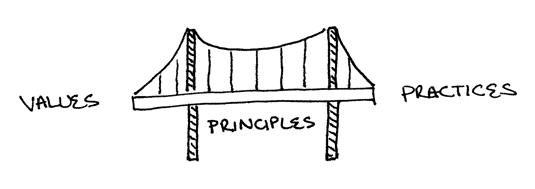
\includegraphics[page=1,width=1.0 \textwidth]{xp_1}
			\caption {\centering \small{Valores, Principios y Pr\'{a}cticas}} \label{figure:chaperII_2}
			\small {Extraido de ``Extreme Programming Explained: Embrace Change, 2nd Edition" de Beck, Kent and Andres - Cynthia, 2004, Copyright by Addison-Wesley Professional.}
		\end{figure}
		
	\subsection{Valores}
		Como dijo Will Rogers, “no es lo que no sabes lo que te mete en problemas. Es lo que sabes que no es así ". El mayor problema que encuentro en lo que la gente``simplemente sab'' sobre el desarrollo de software es que se centran en la acción individual. Lo que realmente importa no es cómo se comporta una persona determinada sino cómo se comportan los individuos como parte de un equipo y como parte de una organización\cite{chap2_extreme_programming}.\\
		Si todos los miembros del equipo deciden centrarse en lo que es importante para el equipo, ¿en qué deberían centrarse? XP adopta cinco valores para guiar el desarrollo: comunicación, simplicidad, retroalimentación, coraje y respeto.
		\subsubsection{Comunicaci\'{o}n}
		Lo que más importa en el desarrollo de software en equipo es la comunicación. Cuando surgen problemas en el desarrollo, la mayoría de las veces alguien ya conoce la solución; pero ese conocimiento no llega a alguien con el poder de hacer el cambio. Esto ocurre internamente cuando ignoro mi intuición, pero los efectos se agravan cuando nos comunicamos entre personas. La comunicación es importante para crear un sentido de equipo y una cooperación eficaz \cite{chap2_extreme_programming}.\\
		Cuando encuentre un problema, pregúntese si el problema fue causado por una falta de comunicación. ¿Qué comunicación necesita ahora para abordar el problema? ¿Qué comunicación necesita para mantenerse fuera de este problema en el futuro?.
		\subsubsection{Simplicidad}
		La simplicidad es el más intensamente intelectual de los valores de XP. Hacer un sistema lo suficientemente simple como para resolver con elegancia solo los problemas de hoy es un trabajo duro. La solución simple de ayer puede estar bien hoy, o puede parecer simplista o compleja. Cuando necesite cambiar para recuperar la simplicidad, debe encontrar un camino desde donde está hasta donde quiere estar.\\
		Los valores están destinados a equilibrarse y apoyarse mutuamente. Mejorar la comunicación ayuda a lograr la simplicidad al eliminar los requisitos innecesarios o diferibles de las preocupaciones actuales. Lograr la simplicidad le brinda mucho menos de qué comunicarse \cite{chap2_extreme_programming}.
		\subsubsection{Retroalimentaci\'{o}n}
		Ninguna dirección fija permanece válida por mucho tiempo; ya sea que estemos hablando de los detalles del desarrollo de software, los requisitos del sistema o la arquitectura del sistema. Las direcciones establecidas antes de la experiencia tienen una vida media especialmente corta. El cambio es inevitable, pero el cambio crea la necesidad de retroalimentación \cite{chap2_extreme_programming}.
		Al estar satisfechos con la mejora en lugar de esperar la perfección instantánea, utilizamos la retroalimentación para acercarnos cada vez más a nuestras metas. La retroalimentación viene de muchas formas:
		\begin{itemize}
			\item Opiniones sobre una idea, tuya o de tus compañeros.
			\item Cómo se ve el código cuando implementas la idea.
			\item Si las pruebas fueron fáciles de escribir.
			\item Si las pruebas se ejecutan.
			\item Cómo funciona la idea una vez que se ha implementado.
		\end{itemize}
		Los equipos de XP se esfuerzan por generar la mayor cantidad de comentarios que puedan manejar lo más rápido posible. Intentan acortar el ciclo de retroalimentación a minutos u horas en lugar de semanas o meses. Cuanto antes lo sepa, antes podrá adaptarse. Es posible que reciba demasiados comentarios. Si el equipo está ignorando comentarios importantes; necesita reducir la velocidad, por frustrante que sea, hasta que pueda responder a los comentarios.
		\subsubsection{Coraje}
		El coraje es una acción eficaz frente al miedo. Algunas personas se han opuesto al uso de la palabra``coraje'', reservándola para lo que hace un soldado que patrulla cuando atraviesa una puerta oscura. Sin pretender disminuir el tipo de coraje físico demostrado por el soldado, es cierto que las personas involucradas en el desarrollo de software sienten miedo. Es la forma en que manejan su miedo lo que dicta si están trabajando como una parte efectiva de un equipo.\\
		A veces, el coraje se manifiesta como un sesgo hacia la acción. Si sabe cuál es el problema, haga algo al respecto. A veces, el coraje se manifiesta como paciencia. Si sabe que hay un problema, pero no sabe cuál es, se necesita valor para esperar a que el problema real surja de manera clara.\\
		El coraje como valor primario sin valores compensatorios es peligroso. Hacer algo sin tener en cuenta las consecuencias no es un trabajo en equipo eficaz. Fomente el trabajo en equipo mirando los otros valores como guía sobre qué hacer cuando tiene miedo \cite{chap2_extreme_programming}.\\
		Si el coraje por sí solo es peligroso, junto con los otros valores es poderoso. El coraje para decir verdades, agradables o desagradables, fomenta la comunicación y la confianza. El valor de descartar las soluciones fallidas y buscar otras nuevas fomenta la sencillez. El coraje de buscar respuestas reales y concretas genera retroalimentación.
		\subsubsection{Respeto}
		Los cuatro valores anteriores apuntan a uno que se encuentra por debajo de la superficie de los otros cuatro: respeto. Si los miembros de un equipo no se preocupan por los demás y por lo que están haciendo, XP no funcionará. Si a los miembros de un equipo no les importa un proyecto, nada puede salvarlo.\\
		Toda persona cuya vida se ve afectada por el desarrollo de software tiene el mismo valor que un ser humano. Nadie es intrínsecamente más valioso que nadie. Para que el desarrollo de software mejore simultáneamente en humanidad y productividad, las contribuciones de cada persona en el equipo deben ser respetadas. Yo soy importante y tú también \cite{chap2_extreme_programming}.
	\subsection{Principios}
		Los valores son demasiado abstractos para guiar directamente el comportamiento. Los documentos largos están destinados a comunicarse, al igual que las conversaciones diarias. ¿Cuál es el más efectivo? La respuesta depende en parte del contexto y en parte de los principios intelectuales. En este caso, el principio de humanidad sugiere que la conversación satisface la necesidad humana básica de conexión y, por tanto, es la forma preferida de comunicación, en igualdad de condiciones. La comunicación escrita es inherentemente más derrochadora. Si bien la comunicación escrita le permite llegar a una gran audiencia, es una comunicación unidireccional. La conversación permite aclaraciones, comentarios inmediatos, lluvia de ideas y otras cosas que no puede hacer con un documento. La comunicación escrita tiende a ser tomada como un hecho o rechazada rotundamente, ninguna de las cuales es una invitación a una mayor comunicación.
		\subsubsection{Humanidad}
			La gente desarrolla software. Este simple e ineludible hecho invalida la mayoría de los consejos metodológicos disponibles. A menudo, el desarrollo de software no satisface las necesidades humanas, no reconoce la fragilidad humana y no aprovecha la fuerza humana. Actuar como si el software no fuera escrito por personas supone un alto costo para los participantes, su humanidad se destruye por un proceso inhumano que no reconoce sus necesidades. Esto tampoco es bueno para los negocios, con los costos y la interrupción de la alta rotación y las oportunidades perdidas para la acción creativa \cite{chap2_extreme_programming}.
			¿Qué necesitan las personas para ser buenos desarrolladores?
			\begin{itemize}
				\item\textbf{Seguridad básica} - estar libre de hambre, daño físico y amenazas a sus seres queridos. El miedo a perder el empleo amenaza esta necesidad.
				\item\textbf{Logro} - la oportunidad y la capacidad de contribuir a su sociedad.
				\item\textbf{Pertenencia} - la capacidad de identificarse con un grupo del que reciben validación y responsabilidad y contribuir a sus objetivos compartidos.
				\item\textbf{Crecimiento} - la oportunidad de ampliar sus habilidades y perspectiva.
				\item\textbf{Intimidad} - la capacidad de comprender y ser comprendido profundamente por los demás.
			\end{itemize}
		\subsubsection{Econ\'{o}micos}
			Alguien tiene que pagar por todo esto. El desarrollo de software que no reconoce la economía corre el riesgo de la victoria vacía de un "éxito técnico". Asegúrese de que lo que está haciendo tenga valor comercial, cumpla con los objetivos comerciales y satisfaga las necesidades comerciales.
		\subsubsection{Beneficio mutuo}
			Cada actividad debe beneficiar a todos los interesados. El beneficio mutuo es el principio XP más importante y el más difícil de cumplir. Siempre hay soluciones para cualquier problema que le cueste a una persona mientras beneficia a otra. Cuando la situación es desesperada, estas soluciones parecen atractivas. Sin embargo, siempre son una pérdida neta, porque la mala voluntad que crean destruye las relaciones que debemos valorar. El negocio de las computadoras es realmente un negocio de personas y mantener las relaciones laborales es importante.\\
			La extensa documentación interna del software es un ejemplo de una práctica que viola el beneficio mutuo. Se supone que debo ralentizar mi desarrollo considerablemente para que alguna persona desconocida en un futuro potencial tenga más facilidad para mantener este código. Puedo ver un posible beneficio para la persona futura en caso de que la documentación aún sea válida, pero ningún beneficio ahora.\\
			XP resuelve el problema de la comunicación con el futuro de formas mutuamente beneficiosas:
			\begin{itemize}
				\item Escribo pruebas automatizadas que me ayudan a diseñar e implementar mejor hoy. Dejo estas pruebas para que las utilicen los futuros programadores. Esta práctica me beneficia ahora y a los mantenedores en el futuro.
				\item Refactorizo cuidadosamente para eliminar la complejidad accidental, dándome satisfacción y menos defectos y haciendo que el código sea más fácil de entender para quienes lo encuentren más adelante.
				\item Elijo nombres de un conjunto coherente y explícito de metáforas que acelera mi desarrollo y hace que el código sea más claro para los nuevos programadores.
			\end{itemize}
		\subsubsection{Auto semejanza}
			Cuando la naturaleza encuentra una forma que funciona, la usa en todos los lugares que puede. El mismo principio se aplica al desarrollo de software: copiar la estructura de una solución en un nuevo contexto, incluso a diferentes escalas.
		\subsubsection{Mejora}
			En el desarrollo de software, ``perfecto'' es un verbo, no un adjetivo. No existe un proceso perfecto. No existe un diseño perfecto. No hay historias perfectas. Sin embargo, puede perfeccionar su proceso, su diseño y sus historias \cite{chap2_extreme_programming}.\\
			Si bien nuestra tecnología mejorada ha eliminado gradualmente el esfuerzo desperdiciado, nuestra mayor rigidez y estructuras sociales especializadas en las organizaciones de desarrollo son cada vez más un desperdicio. La clave para mejorar es conciliar los dos, utilizando la eficiencia tecnológica recién descubierta para permitir nuevas relaciones sociales más efectivas. Ponga a trabajar la mejora sin esperar la perfección. Encuentre un lugar de partida, comience y mejore desde allí.
		\subsubsection{Diversidad}
			Los equipos de desarrollo de software donde todos son iguales, aunque se sientan cómodos, no son efectivos. Los equipos deben reunir una variedad de habilidades, actitudes y perspectivas para ver los problemas y las trampas, pensar en múltiples formas de resolver problemas e implementar las soluciones. Los equipos necesitan diversidad.\\
			El conflicto es el compañero inevitable de la diversidad. No hay conflicto en el sentido de ``nos odiamos y no podemos progresar'', sino en el sentido de “hay dos formas de resolver esto”. ¿Cómo eliges?
			
			Dos ideas sobre un diseño presentan una oportunidad, no un problema. El principio de diversidad sugiere que los programadores deben trabajar juntos en el problema y se deben valorar ambas opiniones.
		\subsubsection{Reflecci\'{o}n}
			Los buenos equipos no solo hacen su trabajo, piensan en cómo están trabajando y por qué están trabajando. Analizan por qué tuvieron éxito o fracasaron. No intentan ocultar sus errores, sino exponerlos y aprender de ellos. Nadie tropieza con la excelencia.
			
			Los ciclos trimestrales y semanales incluyen tiempo para la reflexión en equipo, al igual que la programación por parejas y la integración continua. Pero la reflexión no debe limitarse a las oportunidades ``oficiales''. La conversación con un cónyuge o amigo, las vacaciones y la lectura y las actividades no relacionadas con el software brindan oportunidades individuales para pensar cómo y por qué está trabajando de la manera en que lo hace. Las comidas compartidas y las pausas para el café proporcionan un entorno informal para la reflexión compartida.
			
			La reflexión no es un ejercicio puramente intelectual. Puede obtener información analizando datos, pero también puede aprender de su instinto. Las emociones “negativas” como el miedo, la ira y la ansiedad han proporcionado señales de que algo malo estaba a punto de suceder. Se necesita un esfuerzo para escuchar lo que sus emociones le dicen sobre su trabajo, pero los sentimientos templados por el intelecto son una fuente de conocimiento.
			
			La reflexión puede llevarse demasiado lejos. El desarrollo de software tiene una larga tradición de personas tan ocupadas pensando en el desarrollo de software que no tienen tiempo para desarrollar software. La reflexión viene después de la acción. El aprendizaje es acción reflejada. Para maximizar los comentarios, la reflexión en los equipos de XP se mezcla con la práctica \cite{chap2_extreme_programming}.
		\subsubsection{Flujo}
			El flujo en el desarrollo de software ofrece un flujo constante de software valioso al participar en todas las actividades de desarrollo simultáneamente. Las prácticas de XP están sesgadas hacia un flujo continuo de actividades en lugar de fases discretas.
			
			 Muchos equipos empeoran el problema al tender a responder al estrés haciendo que las partes de valor sean más grandes, desde implementar software con menos frecuencia hasta integrarlo con menos frecuencia. Menos retroalimentación empeora el problema, lo que lleva a una tendencia a fragmentos aún mayores. Cuantas más cosas se aplacen, cuanto mayor es la porción, mayor es el riesgo. En contraste, el principio de flujo sugiere que para mejorar, implemente incrementos más pequeños de valor cada vez con mayor frecuencia.
			
			Algunas tendencias en el desarrollo de software se oponen al concepto de lotes más grandes. La construcción diaria, por ejemplo, está orientada al flujo. Sin embargo, las construcciones diarias son un pequeño paso en el camino hacia la fluidez. No es suficiente que el software se compile y se vincule todos los días; también debería funcionar correctamente todos los días o, mejor aún, varias veces al día \cite{chap2_extreme_programming}.
		\subsubsection{Oportunidad}
			Aprenda a ver los problemas como oportunidades de cambio. Esto no quiere decir que no haya problemas en el desarrollo de software. Sin embargo, la actitud de``supervivencia'' conduce a una resolución de problemas suficiente para salir adelante. Para alcanzar la excelencia, los problemas deben convertirse en oportunidades de aprendizaje y mejora, no solo en la supervivencia.
			
			Es posible que no sepa qué hacer con un problema. Es posible que desee más tiempo para pensar qué hacer. A veces, el deseo de más tiempo es una máscara que se usa para protegerse del miedo a las consecuencias de ponerse en marcha. A veces, sin embargo, la paciencia resuelve un problema por sí sola.
			
			La conversión de problemas en oportunidades se lleva a cabo a lo largo del proceso de desarrollo. Maximiza las fortalezas y minimiza las debilidades. ¿No puede hacer planes precisos a largo plazo? Bien, tenga un ciclo trimestral durante el cual refine sus planes a largo plazo. ¿Una persona sola comete demasiados errores? Bien, programe en parejas. Las prácticas son eficaces precisamente porque abordan los problemas persistentes de las personas que desarrollan software en conjunto.
			
			Cuando empiece a practicar XP, seguramente encontrará problemas. Parte de ser extremo es elegir conscientemente transformar cada problema en una oportunidad: una oportunidad para el crecimiento personal, profundizar las relaciones y mejorar el software \cite{chap2_extreme_programming}.
		\subsubsection{Redundancia}
			 Los problemas críticos y difíciles en el desarrollo de software deben resolverse de varias formas diferentes. Incluso si una solución falla por completo, las otras soluciones evitarán desastres. El costo de la redundancia está más que pagado por los ahorros de no tener el desastre.
			
			Por ejemplo, los defectos corroen la confianza y la confianza es el gran eliminador de desperdicios. Los defectos son un problema crítico y difícil. Los defectos se abordan en XP mediante muchas de las prácticas: programación en pareja, integración continua, sentarse juntos, participación real del cliente e implementación diaria, por ejemplo. Incluso si su socio no detecta un error, alguien más sentado al otro lado de la habitación podría o podría ser detectado por la próxima integración. Algunas de estas prácticas son ciertamente redundantes y presentan algunos de los mismos defectos.
			
			No se puede resolver el problema del defecto con una sola práctica. Es demasiado complejo, con demasiadas facetas y nunca se resolverá por completo. Lo que espera lograr son pocos defectos suficientes para mantener la confianza tanto dentro del equipo como con el cliente \cite{chap2_extreme_programming}.
		\subsubsection{Fracaso}
			Si tiene problemas para tener éxito, falle. ¿No sabes cuál de las tres formas de implementar una historia? Pruébelo de tres formas. Incluso si todos fallan, seguramente aprenderá algo valioso.
			
			¿No es un desperdicio el fracaso? No, no si imparte conocimientos. El conocimiento es valioso y, a veces, difícil de conseguir. La falla puede no ser un desperdicio evitable. Si supiera cuál es la mejor manera de implementar la historia, simplemente la implementaría de esa manera. Dado que aún no conoce la mejor forma, ¿cuál es la forma más barata de averiguarlo?
			
			Esto no tiene la intención de excusar el fracaso cuando realmente sabía mejor. Sin embargo, cuando no sabe qué hacer, arriesgarse a fracasar puede ser el camino más corto y seguro hacia el éxito \cite{chap2_extreme_programming}.
		\subsubsection{Calidad}
			Sacrificar la calidad no es eficaz como medio de control. La calidad no es una variable de control. Los proyectos no van más rápido al aceptar una calidad inferior. No van más despacio al exigir una mayor calidad. Mejorar la calidad a menudo resulta en una entrega más rápida; mientras que la reducción de los estándares de calidad a menudo resulta en una entrega tardía y menos predecible.
			
			Si no puede controlar los proyectos controlando la calidad, ¿cómo puede controlarlos? El tiempo y el costo suelen ser fijos. XP elige el alcance como medio principal de planificación, seguimiento y dirección de proyectos. Dado que el alcance nunca se conoce con precisión de antemano, es una buena palanca. Los ciclos semanales y trimestrales proporcionan puntos explícitos para rastrear y elegir el alcance.
			
			La preocupación por la calidad no es excusa para la inacción. Si no conoce una forma limpia de hacer un trabajo que debe hacerse, hágalo de la mejor manera posible. Si conoce un camino limpio pero tomaría demasiado tiempo, haga el trabajo tan bien como tenga tiempo por ahora. Decida terminar de hacerlo de la manera limpia más tarde. Esto ocurre a menudo durante la evolución arquitectónica, donde tienes que vivir con dos arquitecturas que resuelven el mismo problema mientras haces la transición de una a otra. Entonces, la transición en sí se convierte en una demostración de calidad: realizar un gran cambio de manera eficiente en pasos pequeños y seguros \cite{chap2_extreme_programming}.
		\subsubsection{Pasos pequeños}
			Siempre es tentador hacer grandes cambios en grandes pasos. Después de todo, queda un largo camino por recorrer y poco tiempo para llegar. Un cambio momentáneo tomado de una vez es peligroso. Son las personas a las que se les pide que cambien. El cambio es inquietante. La gente cambia muy rápido.
			
			 Los pasos de bebé no justifican la estasis o el cambio glacial. En las condiciones adecuadas, las personas y los equipos pueden dar muchos pasos pequeños con tanta rapidez que parecen estar dando saltos.
			
			Los pequeños pasos reconocen que la sobrecarga de los pequeños pasos es mucho menor que cuando un equipo retrocede inútilmente ante grandes cambios abortados. Los pequeños pasos se expresan en prácticas como la programación de prueba primero, que avanza una prueba a la vez, y la integración continua, que integra y prueba el valor de algunas horas de cambios a la vez \cite{chap2_extreme_programming}.
		\subsubsection{Aceptar responsabilidad}
			No se puede asignar responsabilidad; solo se puede aceptar. Si alguien intenta responsabilizarte, solo tú puedes decidir si eres responsable o no. Las prácticas reflejan la responsabilidad aceptada, por ejemplo, sugerir que quien se inscribe para hacer un trabajo también la estima. De manera similar, la persona responsable de implementar una historia es en última instancia responsable del diseño, implementación y prueba de la historia. Con la responsabilidad viene la autoridad. Las desalineaciones distorsionan la comunicación del equipo. Cuando un experto en procesos puede decirme cómo trabajar, pero no comparte ese trabajo o sus consecuencias, la autoridad y la responsabilidad están desalineadas.
	\subsection{Pr\'{a}cticas}
		\subsubsection{Pr\'{a}cticas primarias}
			\begin{enumerate}
				\item \textit{\textbf{Sit Together}}\\
				``Sit Together'' predice que cuanto más tiempo presencial tenga, más humano y productivo será el proyecto. Si tienes un proyecto de varios sitios y todo va bien, sigue haciendo lo que estás haciendo. Si tiene problemas, piense en formas de sentarse más juntos, incluso si eso significa viajar.\\
				\item \textit{\textbf{Whole Team}}\\
				Incluir en el equipo a personas con todas las habilidades y perspectivas necesarias para que el proyecto tenga éxito. En realidad, esto no es más que la vieja idea de equipos multifuncionales. El nombre refleja el propósito de la práctica, una sensación de integridad en el equipo, la disponibilidad inmediata de todos los recursos necesarios para tener éxito. Cuando las interacciones intensas son necesarias para la salud del proyecto, quienes interactúan deben identificarse principalmente con el equipo y no con sus funciones.\\
				La gente necesita un sentido de ``equipo'':
				\begin{itemize}
					\item Nosotros pertenecemos.
					\item Estamos en esto juntos.
					\item Apoyamos el trabajo, el crecimiento y el aprendizaje de los demás.
				\end{itemize}
				Lo que constituye un “equipo completo” es dinámico. Si un conjunto de habilidades o actitudes se vuelve importante, traiga al equipo a una persona con estas habilidades. Si alguien ya no es necesario, puede ir a otra parte.
				\item \textit{\textbf{Informative Workspace}}\\
				Haga de su espacio de trabajo su trabajo. Un observador interesado debería poder entrar en el espacio del equipo y tener una idea general de cómo va el proyecto en quince segundos. Debería poder obtener más información sobre problemas reales o potenciales al mirar más de cerca. Muchos equipos implementan esta práctica en parte colocando tarjetas de historias en la pared. Ordenar las tarjetas espacialmente transmite información rápidamente. Si el área "Listo" no recopila tarjetas, ¿qué necesita mejorar el equipo en su planificación, estimación o ejecución? También me preguntaré qué necesitan los clientes para que el alcance deslizante tenga un impacto comercial mínimo. La Figura \ref{figure:chaperII_3} muestra un muro de historias idealizado con historias ordenadas espacialmente.
				\begin{figure}[H]
					\centering
					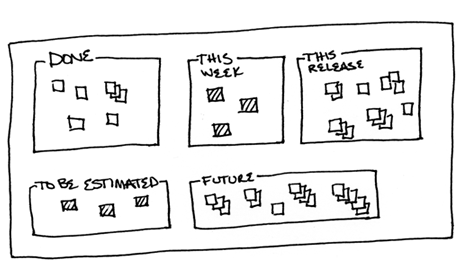
\includegraphics[width=0.5 \textwidth]{xp_2}
					\caption {\centering \small{Historias de usuario en una pared}} \label{figure:chaperII_3}
					\small {Fuente: ``Extreme Programming Explained: Embrace Change, 2nd Ed." por Beck, Kent and Andres - Cynthia, 2004, Copyright by Addison-Wesley Professional.}
				\end{figure}
				El espacio de trabajo (Figura \ref{figure:chaperII_4} ) también debe cubrir otras necesidades humanas. El agua y los bocadillos brindan consuelo y fomentan las interacciones sociales positivas. La limpieza y el orden dejan la mente libre para pensar en los problemas en cuestión. Si bien la programación ocurre en un espacio público, las personas también necesitan privacidad, que puede proporcionarse mediante cubos separados o limitando las horas de trabajo.
				\begin{figure}[H]
					\centering
					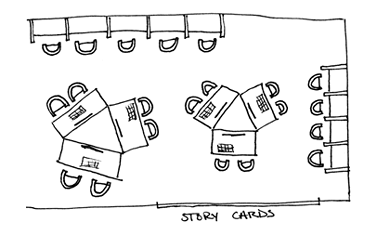
\includegraphics[width=0.5 \textwidth]{xp_3}
					\caption {\centering \small{Espacio de trabajo de un equipo}} \label{figure:chaperII_4}
					\small {Fuente: ``Extreme Programming Explained: Embrace Change, 2nd Ed." por Beck, Kent and Andres - Cynthia, 2004, Copyright by Addison-Wesley Professional.}
				\end{figure}
				
				\item \textit{\textbf{Energized Work}}\\
				Trabaje solo tantas horas como pueda ser productivo y solo tantas horas como pueda mantener. Quemarse improductivamente hoy y estropear el trabajo de los dos días siguientes no es bueno para usted ni para el equipo.
				Es fácil quitar valor a un proyecto de software; pero cuando estás cansado, es difícil reconocer que estás quitando valor\cite{chap2_extreme_programming}.
				
				Cuando esté enfermo, respétese a sí mismo y al resto de su equipo descansando y recuperándose. Cuidar de sí mismo es la forma más rápida de volver al trabajo lleno de energía. También protege al equipo de perder más productividad debido a una enfermedad. Llegar enfermo no demuestra compromiso con el trabajo, porque cuando lo haces no estás ayudando al equipo.
				
				Puede realizar mejoras incrementales en las horas de trabajo. Permanezca en el trabajo la misma cantidad de tiempo, pero adminístrelo mejor. Declare un tramo de dos horas cada día como Código de tiempo. Apague los teléfonos y las notificaciones por correo electrónico, y programe durante dos horas. Eso puede ser una mejora suficiente por ahora y puede preparar el escenario para menos horas de trabajo más adelante \cite{chap2_extreme_programming}.
				\item \textit{\textbf{Pair Programming}}\\
				Escriba todos los programas de producción con dos personas sentadas en una máquina. Configure la máquina para que los socios puedan sentarse cómodamente uno al lado del otro. Mueva el teclado y el mouse hacia adelante y hacia atrás para que se sienta cómodo mientras escribe. La programación en pareja es un diálogo entre dos personas que programan simultáneamente (y analizan, diseñan y prueban) y tratan de programar mejor. Programadores en pareja:
				\begin{itemize}
					\item Mantengan el uno al otro en la tarea.
					\item Haga una lluvia de ideas para mejorar el sistema.
					\item Aclarar ideas.
					\item Tome la iniciativa cuando su pareja esté estancada, reduciendo así la frustración.
					\item Háganse responsables unos a otros de las prácticas del equipo.
				\end{itemize}
				\item \textit{\textbf{Pairing and Personal Space}}\\
				 Diferentes individuos y culturas se sienten cómodos con diferentes cantidades de espacio corporal. Emparejar con un italiano que se comunica mejor cuando está muy cerca es completamente diferente a emparejar con un danés al que le gustan unos pocos pies de espacio personal. Si no es consciente de la diferencia, puede resultar muy incómodo. Se debe respetar el espacio personal para que ambas partes funcionen bien.
				
				La higiene personal y la salud son cuestiones importantes a la hora de emparejar. Cúbrase la boca cuando tosa. No venga a trabajar cuando esté enfermo. Evite las colonias fuertes que puedan afectar a su pareja.
				
				Trabajar juntos de forma eficaz se siente bien. Para algunos, puede ser una nueva experiencia en el lugar de trabajo. Cuando los programadores no son lo suficientemente maduros emocionalmente como para separar la aprobación de la excitación, trabajar con una persona del sexo opuesto puede hacer surgir sentimientos sexuales que no son lo mejor para el equipo. Si estos sentimientos surgen cuando se empareja, deje de emparejarse con la persona hasta que haya asumido la responsabilidad y se haya ocupado de sus sentimientos. Incluso si los sentimientos son mutuos, actuar en consecuencia dañará al equipo. Si desea tener una relación íntima, uno de ustedes debe dejar el equipo para que pueda construir una relación personal en un entorno personal sin confundir la comunicación del equipo con un subtexto sexual. Idealmente, las emociones en el trabajo estarán relacionadas con el trabajo \cite{chap2_extreme_programming}.
				
				\begin{figure}[H]
					\centering
					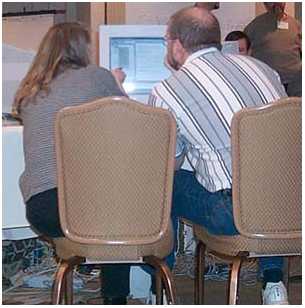
\includegraphics[width=0.5 \textwidth]{xp_4}
					\caption {\centering \small{Programaci\'{o}n en pares}} \label{figure:chaperII_5}
					\small {Fuente: ``Extreme Programming Explained: Embrace Change, 2nd Ed." por Beck, Kent and Andres - Cynthia, 2004, Copyright by Addison-Wesley Professional.}
				\end{figure}
				
				\item \textit{\textbf{Stories}}\\
				El desarrollo de software ha sido mal dirigido por la palabra ``requisito'', definida en el diccionario como ``algo obligatorio u obligatorio''. La palabra tiene una connotación de absolutismo y permanencia, inhibidores de la aceptación del cambio. Y la palabra ``requisito'' es simplemente incorrecta. De mil páginas de ``requisitos'', si implementa un sistema con el 20\% o 10\% o incluso el 5\% correcto, probablemente obtendrá todos los beneficios comerciales previstos para todo el sistema. Entonces, ¿cuál fue el otro 80\%? No ``requisitos''; en realidad no eran obligatorios ni obligatorios.
				
				La estimación temprana es una diferencia clave entre las historias y otras prácticas de requisitos. La estimación brinda a las perspectivas comerciales y técnicas la oportunidad de interactuar, lo que crea valor temprano, cuando una idea tiene el mayor potencial. Cuando el equipo conoce el costo de las funciones, puede dividir, combinar o ampliar el alcance en función de lo que sabe sobre el valor de las funciones.
				
				Dé a las historias nombres cortos además de una breve prosa o una descripción gráfica. Escriba las historias en fichas y colóquelas en una pared que pase con frecuencia. La Figura \ref{figure:chaperII_6}  es una tarjeta de muestra de una historia que deseo que implemente mi programa de escáner. Cada intento que he visto de computarizar historias no ha logrado proporcionar una fracción del valor de tener cartas reales en una pared real. Si necesita informar el progreso a otras partes de la organización en un formato familiar, traduzca las tarjetas a ese formato periódicamente \cite{chap2_extreme_programming}.
				
				\begin{figure}[H]
					\centering
					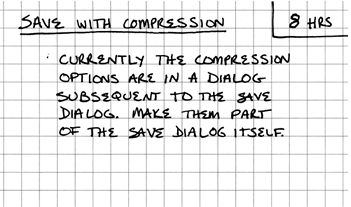
\includegraphics[width=0.5 \textwidth]{xp_5}
					\caption {\centering \small{Tarjeta de historia de usuario}} \label{figure:chaperII_6}
					\small {Fuente: ``Extreme Programming Explained: Embrace Change, 2nd Ed." por Beck, Kent and Andres - Cynthia, 2004, Copyright by Addison-Wesley Professional.}
				\end{figure}
				
				\item \textit{\textbf{Weekly Cycle}}\\
				Planifique el trabajo una semana a la vez. Tenga una reunión al comienzo de cada semana. Durante esta reunión:
				\begin{itemize}
					\item Revise el progreso hasta la fecha, incluyendo cómo el progreso real de la semana anterior coincidió con el progreso esperado.
					\item Haga que los clientes elijan historias de una semana para implementar esta semana.
					\item Divida las historias en tareas. Los miembros del equipo se registran para las tareas y las estiman.
				\end{itemize}
				Comience la semana escribiendo pruebas automatizadas que se ejecutarán cuando se completen las historias. Luego, pase el resto de la semana completando las historias y haciendo que las pruebas pasen. Un equipo orgulloso de su trabajo implementará completamente las historias, no solo hará el trabajo suficiente para que las pruebas pasen. El objetivo es tener software implementable al final de la semana que todos puedan celebrar como progreso.
				\item \textit{\textbf{Quarterly Cycle}}\\
				Planifique el trabajo un cuarto a la vez. Una vez al trimestre, reflexione sobre el equipo, el proyecto, su progreso y su alineación con objetivos más amplios.
				
				Durante la planificación trimestral:
				\begin{itemize}
					\item Identificar los cuellos de botella, especialmente los controlados fuera del equipo.
					\item Inicie las reparaciones.
					\item Planifique el tema o temas para el trimestre.
					\item Elija una cuarta parte de las historias para abordar esos temas.
					\item Concéntrese en el panorama general, donde el proyecto encaja dentro de la organización.
				\end{itemize}
			
				Una temporada es otra escala de tiempo natural y ampliamente compartida para usar en la organización del tiempo para un proyecto. El uso de un trimestre como horizonte de planificación se sincroniza muy bien con otras actividades comerciales que ocurren trimestralmente. Los trimestres también son un intervalo cómodo para la interacción con proveedores y clientes externos.
				La separación de "temas" de "historias" tiene como objetivo abordar la tendencia del equipo a concentrarse y entusiasmarse con los detalles de lo que están haciendo sin reflexionar sobre cómo las historias de esta semana encajan en el panorama general. Los temas también encajan bien en la planificación a mayor escala, como la elaboración de hojas de ruta de marketing \cite{chap2_extreme_programming}.
				\item \textit{\textbf{Slack}}\\
				En cualquier plan, incluya algunas tareas menores que pueden descartarse si se retrasa. Siempre puede agregar más historias más tarde y entregar más de lo prometido. Es importante en un ambiente de desconfianza y promesas incumplidas cumplir con sus compromisos. Algunos compromisos cumplidos contribuyen en gran medida a reconstruir las relaciones.
				\item \textit{\textbf{Ten-Minute Build}}\\
				Cree automáticamente todo el sistema y ejecute todas las pruebas en diez minutos. Una compilación que demore más de diez minutos se usará con mucha menos frecuencia, perdiendo la oportunidad de recibir \textit{feedback}.
				La construcción de diez minutos es ideal. ¿Qué haces en tu camino hacia ese ideal? La declaración de la práctica da tres pistas: construya automáticamente todo el sistema y ejecute todas las pruebas en diez minutos. Si su proceso no está automatizado, ese es el primer lugar para comenzar. Entonces es posible que pueda construir solo la parte del sistema que ha cambiado. Finalmente, es posible que pueda ejecutar solo pruebas que cubran la parte del sistema en riesgo debido a los cambios que realizó. Cualquier suposición sobre qué partes del sistema deben construirse y qué partes deben probarse presenta el riesgo de error. Si está equivocado, puede pasar por alto errores impredecibles con todos sus costos sociales y económicos. Sin embargo, poder probar parte del sistema es mucho mejor que no poder probar ninguno. Las compilaciones automatizadas son mucho más valiosas que las compilaciones que requieren intervención manual. A medida que aumenta el nivel de estrés general, las compilaciones manuales tienden a realizarse con menos frecuencia y menos bien, lo que genera más errores y más estrés. Las prácticas deberían reducir el estrés. Una construcción automatizada se convierte en un alivio del estrés en el momento decisivo. “¿Cometimos un error? Construyamos y veamos\cite{chap2_extreme_programming}”.
				\item \textit{\textbf{Continuous Integration}}\\
				Integre y pruebe los cambios después de no más de un par de horas. La programación en equipo no es un problema de dividir y conquistar. Es un problema de dividir, conquistar e integrar. El paso de integración es impredecible, pero fácilmente puede llevar más tiempo que la programación original. Cuanto más espere para integrarse, más cuesta y más impredecible se vuelve el costo.
				Integrar y construir un producto completo. Si el objetivo es grabar un CD, grabe un CD. Si el objetivo es implementar un sitio web, implemente un sitio web, incluso si es en un entorno de prueba. La integración continua debe ser lo suficientemente completa para que la primera implementación final del sistema no sea gran cosa \cite{chap2_extreme_programming}.
				\item \textit{\textbf{Test-First Programming}}\\
				La comunidad de XP no ha explorado mucho las alternativas a las pruebas para verificar el comportamiento del sistema. Se podrían utilizar herramientas como el análisis estático y la verificación de modelos al estilo de prueba primero. Empieza con una ``prueba'' que dice, por ejemplo, que no hay puntos muertos en el sistema. Después de cada cambio, verifica nuevamente que no haya puntos muertos. Las herramientas de análisis estático que he visto no están diseñadas para usarse de esta manera. Funcionan demasiado lentamente para formar parte del ciclo de programación minuto a minuto. Sin embargo, esto parece ser simplemente una cuestión de enfoque, no una limitación fundamental.				
				En las pruebas continuas, las pruebas se ejecutan en cada cambio de programa, al igual que un compilador incremental se ejecuta en cada cambio en el código fuente. Los fallos de prueba se informan en el mismo formato que los errores del compilador. Las pruebas continuas reducen el tiempo para corregir errores al reducir el tiempo para descubrirlos. Sin embargo, las pruebas deben ejecutarse rápidamente.				
				Las pruebas que escribe mientras codifica test-first tienen la limitación de que toman una microvista del programa: ¿estos dos objetos funcionan bien juntos? A medida que su experiencia crezca, podrá exprimir más y más seguridad en estas pruebas. Debido a su alcance limitado, estas pruebas tienden a ejecutarse muy rápido. Puede ejecutar miles de ellos como parte de la compilación de diez minutos \cite{chap2_extreme_programming}.
				\item \textit{\textbf{Incremental Design}}\\
				Invierta en el diseño del sistema todos los días. Esfuércese por hacer que el diseño del sistema se adapte perfectamente a las necesidades del sistema ese día. Cuando su comprensión del mejor diseño posible salte adelante, trabaje de manera gradual pero persistente para volver a alinear el diseño con su comprensión.
				El consejo para los equipos de XP no es minimizar la inversión en diseño a corto plazo, sino mantener la inversión en diseño en proporción a las necesidades del sistema hasta el momento. La cuestión no es si diseñar o no, la cuestión es cuándo diseñar. El diseño incremental sugiere que el momento más eficaz para diseñar es a la luz de la experiencia.
				Si los pasos pequeños y seguros son cómo diseñar, la siguiente pregunta es en qué parte del sistema se debe mejorar el diseño. La heurística simple que he encontrado útil es eliminar la duplicación. Si tengo la misma lógica en dos lugares, trabajo con el diseño para entender cómo puedo tener solo una copia. Los diseños sin duplicación tienden a ser fáciles de cambiar. No se encuentra en la situación en la que tenga que cambiar el código en varios lugares para agregar una función.
				A medida que más equipos invierten en el diseño diario, notan que los cambios que están realizando son similares independientemente del propósito del sistema. La refactorización es una disciplina de diseño que codifica estos patrones recurrentes de cambios. Estas refactorizaciones pueden ocurrir en cualquier nivel de escala. Pocas decisiones de diseño son difíciles de cambiar una vez tomadas. El resultado son sistemas que pueden comenzar con poco y crecer según sea necesario sin un costo exorbitante \cite{chap2_extreme_programming}.
			\end{enumerate}
		\subsubsection{Pr\'{a}cticas corolarias}
				Las prácticas corolarias son difíciles o peligrosas de implementar antes de completar el trabajo preliminar de las prácticas primarias. Si se comienza a implementar a diario, por ejemplo, sin que la tasa de defectos se acerque a cero (con programación de pares, integración continua y programación de prueba primero); tendrás un desastre en tus manos. Confíe en su olfato sobre lo que necesita mejorar a continuación. Si alguna de las siguientes prácticas parece apropiada, pruébela. Podría funcionar o podría descubrir que tiene más trabajo por hacer antes de poder usarlo para mejorar su proceso de desarrollo.
				\begin{itemize}
					\item Real Customer Involvement
					\item Incremental Deployment
					\item Team Continuity
					\item Shrinking Teams
					\item Root-Cause Analysis
					\item Shared Code
					\item Code and Tests
					\item Single Code base
					\item Daily Deployment
					\item Negotiated Scope Contract
					\item Pay-Per-Use
				\end{itemize}
	\subsection{Planificaci\'{o}n}
				Planificar en XP es como ir de compras. Imagínese que entra en una tienda de comestibles con \$ 100 en el bolsillo. Los artículos en los estantes tienen un precio adjunto. Algunos elementos que necesita; otros no; y otros que desee, pero no se ajustan a su presupuesto. Si llega a la caja con \$ 101 en comida, tendrá que devolver algo. Su trabajo al comprar es gastar sus \$ 100 sabiamente, comprando lo que necesita y tanto como sea posible.
				
				En XP, las compras son las historias. Los precios son las estimaciones adjuntas a las historias. El presupuesto es la cantidad de tiempo disponible. La fecha de implementación deseada generalmente se establece al principio de un proyecto, para que sepa cuánto tiene que gastar en historias. Si tiene doscientos pares de horas en su bolsillo y tiene cuatrocientos pares de horas de historias en su carrito, elija el conjunto de historias más valioso que sume hasta doscientos pares de horas. De lo contrario, todos saben que tiene más en el carrito de lo que puede pagar.	
				
				Parte de la planificación es decidir qué hacer a continuación entre todas las posibilidades. La planificación es complicada porque las estimaciones del costo y el valor de las historias son inciertas. La información en la que basa estas decisiones cambia. Usamos la retroalimentación para mejorar nuestras estimaciones y tomar decisiones lo más tarde posible para que se basen en la mejor información posible. Es por eso que la planificación es una actividad diaria, semanal y trimestral en XP. El plan puede cambiar para adaptarse a los hechos a medida que surgen.
				Los planes no son predicciones del futuro. En el mejor de los casos, expresan todo lo que sabe hoy sobre lo que podría suceder mañana. Su incertidumbre no niega su valor. Los planes le ayudan a coordinarse con otros equipos. Los planes le brindan un lugar para comenzar. Los planes ayudan a todos en el equipo a tomar decisiones alineadas con los objetivos del equipo \cite{chap2_extreme_programming}.
				
				Para estimar una historia, imagina, dado todo lo que sabes sobre historias similares, cuántas horas o días le tomará a un par completar la historia. “Completo” significa listo para el despliegue; incluyendo todas las pruebas, implementación, refactorización y discusiones con los usuarios. A medida que aumente su conocimiento de historias similares, sus estimaciones mejorarán. Las estimaciones se basan en un par razonable que trabaja en la historia. Algunos pares pueden ser mejores y otros peores, pero si todos se turnan para estimar, todos deberían promediar al final.
				
				Al principio, estas estimaciones pueden ser tremendamente erróneas. Las estimaciones basadas en la experiencia son más precisas. Es importante recibir comentarios lo antes posible para mejorar sus estimaciones. Si tiene un mes para planificar un proyecto en detalle, dedíquelo a desarrollar cuatro iteraciones de una semana mientras mejora sus estimaciones. Si tiene una semana para planificar un proyecto, realice cinco iteraciones de un día. Los ciclos de retroalimentación le brindan información y la experiencia para realizar estimaciones precisas. Obtenga esta experiencia lo antes posible para mejorar sus estimaciones.
	\subsection{Diseño}
				El diseño incremental es una forma de entregar funcionalidad temprana y continuar brindando funcionalidad semanalmente durante la vida del proyecto. XP lleva el incrementalismo del diseño al límite, lo que sugiere que los proyectos se ejecutan con mayor fluidez si el diseño es parte del trabajo diario \cite{chap2_extreme_programming}.
				
				En el mundo físico, las transformaciones individuales cuestan demasiado para que el diseño incremental funcione bien. Las etapas intermedias tienen muy poco valor o los cambios son demasiado costosos (las piezas se destruyen y es costoso duplicarlas en el proceso de reconstrucción).Incluso las estructuras físicas se someten a un diseño y construcción incrementales, y la experiencia de la estructura existente informa la siguiente etapa del diseño de formas que la especulación no puede \cite{chap2_extreme_programming}.
				
				Parte de lo que hace que el diseño incremental sea valioso en el software es que a menudo escribimos aplicaciones por primera vez. Incluso si esta es la enésima variación de un tema, siempre hay una mejor manera de diseñar el software. Como el diseño tiene influencia y las ideas de diseño mejoran con la experiencia, la paciencia es una de las habilidades más valiosas que puede poseer un diseñador de software. Hay un arte en diseñar lo suficiente para obtener retroalimentación y luego usar esa retroalimentación para mejorar el diseño lo suficiente como para obtener la siguiente ronda de retroalimentación \cite{chap2_extreme_programming}.
				
				Los siguientes gráficos nos ayudarán a visualizar por sí mismo cuándo debe diseñar. El eje vertical del gráfico es la calidad del diseño. Hay una línea horizontal para la calidad mínima del diseño necesaria para el éxito. El diseño de software es curioso, ya que generalmente hay muchos diseños que son lo suficientemente buenos para que el software tenga éxito. La calidad del diseño no garantiza el éxito, pero el fracaso del diseño puede garantizar el fracaso \cite{chap2_extreme_programming}.
				
				Cada gráfico tendrá tres puntos, uno para cómo diseñarías ``por instinto'', otro para cómo diseñarías si pensaras mucho en el diseño y otro para cómo diseñarías a la luz de la experiencia. La relación de los tres puntos y la ubicación del umbral de diseño mínimo indicará si diseñar por adelantado es una opción para usted, o si estaría mejor con un diseño incremental \cite{chap2_extreme_programming}.
				
				La figura \ref{figure:chaperII_10} es un gráfico en el que el diseño puramente instintivo es suficiente. Cualquier diseño antiguo servirá. Puede seguir adelante y diseñar hoy y tener éxito.
				\begin{figure}[H]
					\centering
					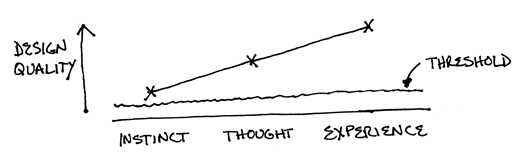
\includegraphics[width=0.8 \textwidth]{xp_9}
					\caption {\centering \small{Cualquier diseño antiguo servirá}} \label{figure:chaperII_10}
					\small {Fuente: ``Extreme Programming Explained: Embrace Change, 2nd Ed." por Beck, Kent and Andres - Cynthia, 2004, Copyright by Addison-Wesley Professional.}
				\end{figure}
				
				La Figura \ref{figure:chaperII_11} es un escenario en el que la cuestión de cuándo diseñar no es tan clara. Pensar detenidamente conduciría a una respuesta suficientemente buena, pero la experiencia conduciría a una mejor respuesta. No tiene la opción de no diseñar en absoluto, porque el diseño inconsciente conducirá al fracaso. ¿Debería hacer la mayor parte de su inversión en diseño ahora o esperar hasta tener algo de experiencia?
				
				\begin{figure}[H]
					\centering
					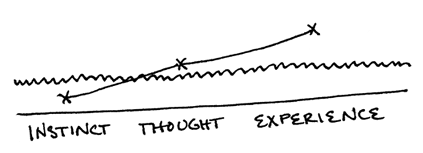
\includegraphics[width=0.7 \textwidth]{xp_10}
					\caption {\centering \small{Se necesita algo de pensamiento o experiencia en diseño}} \label{figure:chaperII_11}
					\small {Fuente: ``Extreme Programming Explained: Embrace Change, 2nd Ed." por Beck, Kent and Andres - Cynthia, 2004, Copyright by Addison-Wesley Professional.}
				\end{figure}
				
				La Figura \ref{figure:chaperII_12} es un caso donde diseño incremental es inevitable. Ninguna cantidad de pensamiento sin experiencia resultará en un diseño que sea lo suficientemente bueno. Solo la experiencia dará como resultado la comprensión suficiente para producir un diseño suficientemente bueno.
				
				\begin{figure}[H]
					\centering
					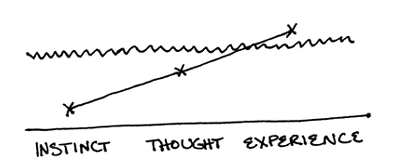
\includegraphics[width=0.7 \textwidth]{xp_11}
					\caption {\centering \small{Ninguna cantidad de pensamiento puro será suficiente}} \label{figure:chaperII_12}
					\small {Fuente: ``Extreme Programming Explained: Embrace Change, 2nd Ed." por Beck, Kent and Andres - Cynthia, 2004, Copyright by Addison-Wesley Professional.}
				\end{figure}
								
				Un factor a tener en cuenta para decidir cuándo diseñar es el valor disponible a través de las diferentes estrategias. Si el pensamiento puro crea la mayor parte del valor sin retroalimentación (Figura \ref{figure:chaperII_13}), diseñar antes tiene más sentido. Si la experiencia crea la mayor parte del valor (Figura \ref{figure:chaperII_14}), diseñar solo lo suficiente hoy para comenzar y luego diseñar principalmente a la luz de la experiencia tiene más sentido.
				
				\begin{figure}[H]
					\centering
					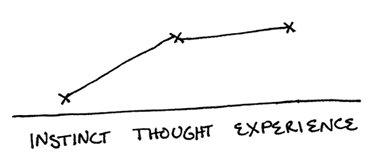
\includegraphics[width=0.7 \textwidth]{xp_12}
					\caption {\centering \small{La experiencia no ayuda}} \label{figure:chaperII_13}
					\small {Fuente: ``Extreme Programming Explained: Embrace Change, 2nd Ed." por Beck, Kent and Andres - Cynthia, 2004, Copyright by Addison-Wesley Professional.}
				\end{figure}
				\begin{figure}[H]
					\centering
					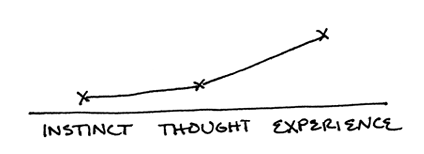
\includegraphics[width=0.7 \textwidth]{xp_13}
					\caption {\centering \small{Mucho que aprender de la experiencia}} \label{figure:chaperII_14}
					\small {Fuente: ``Extreme Programming Explained: Embrace Change, 2nd Ed." por Beck, Kent and Andres - Cynthia, 2004, Copyright by Addison-Wesley Professional.}
				\end{figure}
				
				\subsubsection{Simplicidad}
				Los equipos de XP prefieren soluciones simples siempre que sea posible. A continuación, se muestran cuatro criterios utilizados para evaluar la simplicidad de un diseño.
					\begin{itemize}
						\item \textbf{Apropiado para la audiencia destinataria}. No importa lo brillante y elegante que sea una pieza de diseño; si las personas que necesitan trabajar con él no lo entienden, no es sencillo para ellos.
						\item\textbf{Comunicativo.} Cada idea que necesita ser comunicada está representada en el sistema. Como las palabras de un vocabulario, los elementos del sistema se comunican con los futuros lectores.
 						\item \textbf{Factorizado.} La duplicación de lógica o estructura dificulta la comprensión y modificación del código.
						\item \textbf{Mínimo.} Dentro de las tres restricciones anteriores, el sistema debe tener la menor cantidad de elementos posible. Menos elementos significa menos para probar, documentar y comunicar.
					\end{itemize}
					
	\subsection{Pruebas}
				Los defectos destruyen la confianza necesaria para un desarrollo de software eficaz. Los clientes deben poder confiar en el software. Los gerentes deben poder confiar en los informes de progreso. Los programadores deben poder confiar entre ellos. Los defectos destruyen esta confianza. Sin confianza, las personas pasan gran parte de su tiempo defendiéndose de la posibilidad de que otra persona haya cometido un error \cite{chap2_extreme_programming}.
				
				Aquí está el dilema en el desarrollo de software: los defectos son costosos, pero eliminarlos también es costoso. Sin embargo, la mayoría de los defectos terminan costando más de lo que hubiera costado prevenirlos. Los defectos son costosos cuando ocurren, tanto los costos directos de arreglar los defectos como los costos indirectos debido a relaciones dañadas, negocios perdidos y tiempo de desarrollo perdido. Las prácticas de XP tienen como objetivo comunicarse claramente para que no surjan defectos en primer lugar y, cuando lo hagan, asegurarse de que el equipo las utilice para aprender a evitar problemas similares en el futuro \cite{chap2_extreme_programming}.
				
				Siempre habrá defectos. Surgirán circunstancias inesperadas. En situaciones novedosas e imprevistas, es probable que el software haga algo que el autor no habría tenido la intención de haber sabido de antemano la situación.
				
				Los niveles aceptables de defectos varían. Uno de los objetivos del desarrollo es reducir la aparición de defectos a un nivel económicamente sostenible. Este nivel es diferente para diferentes tipos de software.
				
				Otro objetivo del desarrollo es reducir la aparición de defectos a un nivel en el que la confianza pueda crecer razonablemente en el equipo. La inversión en la reducción de defectos tiene sentido como inversión en el trabajo en equipo. Los errores introducidos por un programador dificultan que todos los demás hagan su trabajo. Cada error de un miembro del equipo que afecta a otro le cuesta tiempo, energía y confianza al equipo. El buen trabajo y el buen trabajo en equipo fortalecen la moral y la confianza. Si puede respetar y confiar en sus colegas, podrá ser más productivo y disfrutar más de su trabajo. Ocultar errores para protegerse, aunque a veces parece necesario, es una enorme pérdida de tiempo y energía. La confianza da energía a los participantes. Nos sentimos bien cuando las cosas funcionan bien. Necesitamos estar seguros para experimentar y cometer errores. Necesitamos pruebas para responsabilizarnos de nuestra experimentación, de modo que podamos estar seguros de que no estamos haciendo daño \cite{chap2_extreme_programming}.
				
				El aumento del costo de los defectos (DCI) es el segundo principio que se aplica en XP para aumentar la rentabilidad de las pruebas. DCI es una de las pocas verdades verificadas empíricamente sobre el desarrollo de software: cuanto antes encuentre un defecto, más barato será repararlo. Si encuentra un defecto después de una década de implementación, tendrá que reconstruir una gran cantidad de historia y contexto para averiguar qué se suponía que debía hacer el código en primer lugar, cuáles de esas suposiciones son erróneas y qué debería corregirse. por lo que el resto del programa (presumiblemente correcto) permanece inalterado. Detecte el mismo defecto en el momento en que se crea y el costo de reparación será mínimo \cite{chap2_extreme_programming}.
				
				DCI implica que los estilos de desarrollo de software con ciclos de retroalimentación largos (Figura \ref{figure:chaperII_7}) serán costosos y tendrán muchos defectos residuales. El presupuesto para encontrar y reparar defectos es limitado. Cuanto mayor sea el costo de búsqueda y reparación de defectos, más defectos permanecerán en el código implementado.
				
				\begin{figure}[H]
					\centering
					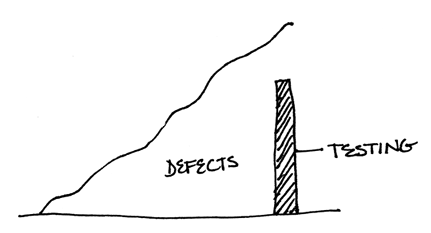
\includegraphics[width=0.6 \textwidth]{xp_6}
					\caption {\centering \small{Las pruebas tardías y costosas dejan muchos defectos}} \label{figure:chaperII_7}
					\small {Fuente: ``Extreme Programming Explained: Embrace Change, 2nd Ed." por Beck, Kent and Andres - Cynthia, 2004, Copyright by Addison-Wesley Professional.}
				\end{figure}
			
			XP usa DCI a la inversa para reducir tanto el costo de reparar defectos como el número de defectos implementados. Al incorporar las pruebas automatizadas al ciclo interno de la programación (Figura \ref{figure:chaperII_8}), XP intenta corregir los defectos de manera más rápida y económica. Esto les da a los equipos de XP la oportunidad de desarrollar software a bajo costo con muy pocos defectos para los estándares de sus contemporáneos.
			
			\begin{figure}[H]
				\centering
				
\includegraphics[width=0.7 \textwidth]{xp_7}
				\caption {\centering \small{Las pruebas frecuentes reducen los costos y los defectos}} \label{figure:chaperII_8}
				\small {Fuente: ``Extreme Programming Explained: Embrace Change, 2nd Ed." por Beck, Kent and Andres - Cynthia, 2004, Copyright by Addison-Wesley Professional.}
			\end{figure}
		
		Si los programadores escriben pruebas, es posible que aún se necesite otra perspectiva del sistema. Un programador o incluso una pareja aportan a su código y prueban un punto de vista singular sobre el funcionamiento del sistema, perdiendo parte del valor de la doble verificación. La verificación doble funciona mejor cuando dos procesos de pensamiento distintos llegan a la misma respuesta. Por eso es peligroso copiar los resultados de un cálculo como su valor esperado. Solo lo has pensado una vez. Es mucho mejor calcular un ejemplo a mano para tener una segunda perspectiva \cite{chap2_extreme_programming}.
		
		Para obtener todos los beneficios de la doble verificación, en XP hay dos conjuntos de pruebas: un conjunto está escrito desde la perspectiva de los programadores, probando los componentes del sistema de manera exhaustiva, y otro conjunto está escrito desde la perspectiva de los clientes o usuarios, probando el funcionamiento del sistema en su conjunto. Estas pruebas se comprueban entre sí. Si las pruebas de los programadores son perfectas, las pruebas del cliente no detectarán ningún error \cite{chap2_extreme_programming}.
		
		La inmediatez de las pruebas en XP también implica que las pruebas deben automatizarse. Con el tiempo, al mejorar el diseño y personalizar las herramientas de desarrollo, el equipo reduce el costo de automatizar las pruebas hasta el punto de que todas las pruebas están automatizadas. Las pruebas automatizadas rompen el ciclo de estrés (Figura \ref{figure:chaperII_9}).
		
		\begin{figure}[H]
			\centering
			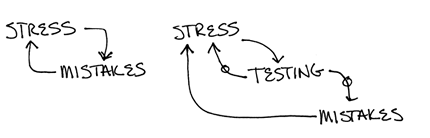
\includegraphics[width=0.7 \textwidth]{xp_8}
			\caption {\centering \small{El ciclo de Stress}} \label{figure:chaperII_9}
			\small {Fuente: ``Extreme Programming Explained: Embrace Change, 2nd Ed." por Beck, Kent and Andres - Cynthia, 2004, Copyright by Addison-Wesley Professional.}
		\end{figure}
		
		En XP, las pruebas son tan importantes como la programación. Escribir y ejecutar las pruebas le da al equipo la oportunidad de hacer un trabajo del que puede estar orgulloso. La ejecución de pruebas le da al equipo una base válida para la confianza a medida que avanza rápidamente en direcciones imprevistas. Las pruebas aportan valor al desarrollo fortaleciendo las relaciones de confianza dentro del equipo y con los clientes.
%------------------------------------------------------------------------------------------------------------------
%-------------------------------Tecnologias backend para la integracion--------------------------------------------
%------------------------------------------------------------------------------------------------------------------
\section{Tecnolog\'{i}as BackEnd para la integraci\'{o}n del proyecto Saiku Analytics}
	\subsection{Lenguaje de programaci\'{o}n Java}
		El lenguaje de programación Java ™ es un lenguaje orientado a objetos de uso general, concurrente, fuertemente tipado y basado en clases. Normalmente se compila con el conjunto de instrucciones de código de bytes y el formato binario definido en la Especificación de máquina virtual de Java \cite{chap2_java}.
	\subsection{Java Specification Requests(JSRs)}
		Las solicitudes de especificación de Java (JSR) son las descripciones reales de las especificaciones propuestas y finales para la plataforma Java \cite{chap2_jsr}.
		\subsubsection{JSR-366}
			Este JSR es para desarrollar Java EE 8, la próxima versión de Java Platform, Enterprise Edition.
			El enfoque principal de esta versión es el soporte para HTML5 y el estándar emergente HTTP 2.0; simplificación mejorada e integración de beans gestionados; e infraestructura mejorada para aplicaciones que se ejecutan en la nube.
			Desde su inicio, la plataforma Java EE ha tenido como objetivo liberar al desarrollador de las tareas de infraestructura comunes a través de su modelo basado en contenedores y la abstracción del acceso a los recursos. En lanzamientos recientes, la plataforma ha simplificado considerablemente las API para acceder a los servicios de contenedor al tiempo que amplía la gama de servicios disponibles. En esta versión, nuestro objetivo es continuar en la dirección de una simplificación mejorada, al tiempo que ampliamos el rango de la plataforma Java EE para abarcar tecnologías emergentes en el espacio web y en la tecnología en la nube \cite{chap2_jsr_366}.
		\subsubsection{JSR-47}
			Una especificación para las API de registro dentro de la plataforma JavaTM. Estas API serán adecuadas para registrar eventos desde la plataforma Java y desde las aplicaciones Java \cite{chap2_jsr_47}.
			
			Se prevé que:
			\begin{itemize}
				\item Será posible habilitar o deshabilitar el registro en tiempo de ejecución.
				\item Será posible controlar el registro con una granularidad bastante fina, de modo que el registro se pueda habilitar o deshabilitar para una funcionalidad específica.
				\item Las API de registro permitirán el registro de los servicios de registro en tiempo de ejecución, por lo que terceros pueden agregar nuevos servicios de registro.
				\item Será posible proporcionar servicios de puente que conecten las API de registro de Java a los servicios de registro existentes (por ejemplo, registros del sistema operativo).
				\item Cuando corresponda, las API de registro también admitirán la visualización de mensajes de alta prioridad a los usuarios finales.
			\end{itemize}
		\subsubsection{JSR-338}
			La API de persistencia de Java es la API de Java para la gestión de la persistencia y el mapeo de objetos / relacionales en entornos Java EE y Java SE. Proporciona una función de mapeo relacional / de objetos para el desarrollador de aplicaciones Java que utiliza un modelo de dominio Java para administrar una base de datos relacional.
			El propósito de la especificación Java Persistence 2.1 es ampliar la API de persistencia Java para incluir características adicionales solicitadas por la comunidad \cite{chap2_jsr_338}.
		\subsubsection{JSR-346}
			Contexts and Dependency Injection for Java EE (CDI) 1.0 se introdujo como parte de la plataforma Java EE 6 y se ha convertido rápidamente en uno de los componentes más importantes y populares de la plataforma. CDI define un poderoso conjunto de servicios complementarios que ayudan a mejorar la estructura del código de la aplicación \cite{chap2_jsr_346}.
			\begin{itemize}
				\item Un ciclo de vida bien definido para objetos con estado vinculados a contextos de ciclo de vida, donde el conjunto de contextos es extensible
				\item Un mecanismo de inyección de dependencias sofisticado y con seguridad de tipos, que incluye \item la capacidad de seleccionar dependencias en el momento del desarrollo o la implementación, sin una configuración detallada
				\item Soporte para la modularidad de Java EE y la arquitectura de componentes de Java EE: la estructura modular de una aplicación Java EE se tiene en cuenta al resolver las dependencias entre los componentes de Java EE.
				\item Integración con el lenguaje de expresión unificado (EL), lo que permite que cualquier objeto contextual se utilice directamente dentro de una página JSF o JSP
				\item La capacidad de decorar objetos inyectados.
				\item La capacidad de asociar interceptores a objetos a través de enlaces de interceptores de tipo seguro.
				\item Un modelo de notificación de eventos
				\item Un contexto de conversación web además de los tres contextos web estándar definidos por la especificación Java Servlets.
				\item Un SPI que permite que las extensiones portátiles se integren limpiamente con el contenedor
			\end{itemize}
		\subsubsection{JSR-369}
				El objetivo principal de este JSR es mostrar la compatibilidad con el próximo estándar IETF HTTP / 2 a los usuarios de la API de Servlet. Un objetivo secundario es actualizar la API de Servlet para lograr el cumplimiento de las nuevas funciones en HTTP 1.1, así como responder a las opiniones de la comunidad.
				HTTP / 2 todavía está en desarrollo activo en un grupo de trabajo (WG) de IETF, sin embargo, se espera que se complete mucho antes de la fecha de finalización de Java EE 8. Si bien en general es una mala idea rastrear un objetivo en movimiento como como una especificación IETF desarrollada activamente, varios factores mitigan el riesgo en este caso \cite{chap2_jsr_369}.
		\subsubsection{JSR-370}
			Los eventos enviados por el servidor (SSE) es una nueva tecnología definida como parte del conjunto de recomendaciones HTML5 para que un cliente (por ejemplo, un navegador) obtenga actualizaciones automáticamente de un servidor a través de HTTP. Se emplea comúnmente para transmisiones de datos de flujo unidireccional en las que un servidor actualiza a un cliente periódicamente o cada vez que ocurre un evento.
			
			JAX-RS 2.0 introdujo la noción de procesamiento asincrónico tanto para el cliente como para las API del servidor. Sin embargo, el procesamiento asincrónico por sí solo no puede cumplir todas las promesas de una arquitectura moderna sin la ayuda de I/O sin bloqueo. Si solo está disponible el bloqueo de I/O, el procesamiento asincrónico simplemente empuja el problema de un hilo al siguiente; esto es similar a pedir prestado a una persona para pagar a otra, el problema no se resuelve realmente, solo se aplaza. Por lo tanto, es necesario admitir I/O sin bloqueo para lograr un alto rendimiento y administrar de manera eficiente recursos como subprocesos.\\
			\cite{chap2_jsr_370}
		\subsubsection{JSR-371}
		En un marco basado en acciones, las solicitudes HTTP se enrutan a los controladores y se convierten en acciones mediante el código de la aplicación; en un marco basado en componentes, las solicitudes HTTP se agrupan y, por lo general, cada componente las maneja de manera independiente. El marco definido por este JSR cae en la categoría basada en acciones y, por lo tanto, no pretende ser un reemplazo del JSF basado en componentes, sino simplemente un enfoque diferente para construir aplicaciones web en la plataforma Java EE.
	\subsection{\textit{Spring Framework}}
			\textit{Spring Framework} proporciona un modelo integral de programación y configuración para aplicaciones empresariales modernas basadas en Java, en cualquier tipo de plataforma de implementación.
			Un elemento clave de Spring es el soporte de infraestructura a nivel de aplicación: \textit{Spring} se enfoca en la "plomería" de aplicaciones empresariales para que los equipos puedan enfocarse en la lógica de negocios a nivel de aplicación, sin vínculos innecesarios con entornos de implementación específicos \cite{chap2_spring}, Spring tiene las siguientes caractesr\'{i}sticas.
			
			\begin{itemize}
				\item Tecnologías principales: inyección de dependencia, eventos, recursos, i18n, validación, enlace de datos, conversión de tipos, SpEL, AOP.
				\item Acceso a datos: transacciones, soporte DAO, JDBC, ORM, Marshalling XML.
				\item Marcos web Spring MVC y Spring WebFlux.
				\item Integración: remoto, JMS, JCA, JMX, correo electrónico, tareas, programación, caché.
				\item Lenguajes de programaci\'{o}n: Kotlin, Groovy, lenguajes dinámicos.
			\end{itemize}
		\subsubsection{\textit{Spring security}}
				\lipsum[1-2]
	\subsection{Maven}
			\lipsum[1-2]
	\subsection{Mondrian}
			\lipsum[1-2]
	\subsection{Git}
			\lipsum[1-2]
	\subsection{Enunciate}
			\lipsum[1-2]
%------------------------------------------------------------------------------------------------------------------
%-------------------------------Tecnologias backend para la integracion--------------------------------------------
%------------------------------------------------------------------------------------------------------------------
\section{Tecnolog\'{i}as FrontEnd para la integraci\'{o}n
		 del proyecto Saiku Analytics}
		\lipsum[1-2]
	\subsection{ECMAScript6 (ES6)}
			\lipsum[1-2]
	\subsection{HTML5}
			\lipsum[1-2]
	\subsection{Javascript}
			\lipsum[1-2]
	\subsection{Css}
			\lipsum[1-2]
	\subsection{Backbone}
			\lipsum[1-2]
	\subsection{Node.js}
			\lipsum[1-2]
	\subsection{CCC-Charts}
			\lipsum[1-2]
\end{spacing}
		
		
		
%JCache (JSR-107)
%Java API for JSON Binding (JSR-367)
%Model View Controller (MVC) (JSR-371)
%Java API for WebSocket
%Java API for JSON Processing (JSON-P)
%Java API for RESTful Web Services (JAX-RS) JSR-370
%JavaServer Faces (JSF)
%Java Servlet JSR-369
%Expression Language (EL)
%Interceptors
%Java Message Service (JMS)
%Concurrency Utilities for Java EE
%Batch Applications for the Java Platform
%Contexts and Dependency Injection for Java EE (CDI) JSR-346
%Bean Validation
%Common Annotations
%Java Connector Architecture
%Java Transaction API (JTA)
%Java Persistence API (JPA) JSR-338
%Enterprise JavaBeans (EJB)
%JavaServer Pages (JSP)
%Web-Profile